%% LyX 2.3.6.1 created this file.  For more info, see http://www.lyx.org/.
%% Do not edit unless you really know what you are doing.
\documentclass[english]{scrartcl}
\usepackage[T1]{fontenc}
\usepackage[latin9]{inputenc}
\setcounter{tocdepth}{2}
\usepackage{babel}
\usepackage{float}
\usepackage{fancybox}
\usepackage{calc}
\usepackage{bm}
\usepackage{amsmath}
\usepackage{graphicx}
\PassOptionsToPackage{normalem}{ulem}
\usepackage{ulem}
\usepackage[unicode=true,pdfusetitle,
 bookmarks=true,bookmarksnumbered=false,bookmarksopen=false,
 breaklinks=false,pdfborder={0 0 1},backref=false,colorlinks=false]
 {hyperref}

\makeatletter

%%%%%%%%%%%%%%%%%%%%%%%%%%%%%% LyX specific LaTeX commands.
%% Because html converters don't know tabularnewline
\providecommand{\tabularnewline}{\\}

\makeatother

\usepackage{listings}
\renewcommand{\lstlistingname}{Listing}

\begin{document}
\title{xQSim Manual: v2.0}
\author{Peter D. Drummond, Alexander S. Dellios}

\maketitle
\newpage{}

\tableofcontents{}

\newpage{}

\section{Introduction}

Large, network based experiments in quantum optics are becoming increasingly
common, pushing the development of networks to ever large sizes. These
optical linear networks have a variety of applications such as quantum
computers implementing a type of random-number generation \cite{Aaronson2011,AaronsonArkhipov2013LV,Aaronson:2014,Hamilton2017PhysRevLett.119.170501,quesada2018gaussian,kruse2019detailed}
and large scale interferometers producing output measurements below
the shot noise limit \cite{Motes2015_PRL114,Su2017Multiphoton}. 

Many implementations use nonclassical inputs \cite{Reid1986violations}
such as squeezed states or number states. These are not mathematically
representable as a classical, positive, non-singular Glauber-Sudarshan
phase-space distribution \cite{Glauber_1963_P-Rep,Sudarshan_1963_P-Rep}. 

Recently, large networks employed as quantum computers have been used
to claim quantum computational advantage \cite{arute2019quantum,zhong2020quantum,Zhong2021Phase,madsenQuantumComputationalAdvantage2022}.
This leads to a theoretical challenge: how does one check hardware
operation? Are the random numbers generated correctly? Do they follow
the expected probability distribution?

Traditional number-state validation methods are only practical for
small scale networks, since they use an exponentially large basis
set. This rules out direct calculations, due to the finite size, computational
time and precision of a digital computer. Although more feasible,
even Monte-Carlo methods take an exponentially long time digitally
\cite{bulmerBoundaryQuantumAdvantage2022a}.

Other methods utilize marginal probabilities of the expected distribution,
which are calculable \cite{villalonga2021efficient,ohSpoofingCrossEntropy2022a}.
Although scalable, such methods cannot verify higher-order correlations
generated in the network. Therefore, these methods can only validate
part of a larger picture. 

For Gaussian boson sampling with linear networks, other methods using
quantum phase-space exist. These do allow comparisons of theory and
experiment for large, nonclassical networks, simulating all possible
correlations generated by an experiment. A computational implementation
is necessary, however. xQSim - meaning e\textbf{x}tensible \textbf{Q}uantum
\textbf{Sim}ulations using phase-space representations - is a software
package that does this. 

While xQSim is able to compare theoretical predictions with experimental
data, it cannot generate a direct random output of photon counts.
This is the task implemented by experiments \cite{zhong2020quantum,Zhong2021Phase,madsenQuantumComputationalAdvantage2022}
and some validation methods \cite{villalonga2021efficient}. However,
there is extensive theory suggesting that such brute-force computations
are \#P hard \cite{Aaronson2011,AaronsonArkhipov2013LV,Aaronson:2014,lund2014boson,Hamilton2017PhysRevLett.119.170501,quesada2018gaussian,kruse2019detailed},
and therefore our code implements a completely different approach.

To do this, we employ three phase-space simulation methods: the positive
P-distribution \cite{Drummond_generalizedP1980} ($method=1$), the
Wigner distribution \cite{Wigner_1932} ($method=2$), provided it
has a positive distribution for the corresponding input state, and
the Husimi Q-function \cite{Husimi1940} ($method=3$). 

The present code distribution can simulate multidimensional photon
probabilities, photon number correlations and quadrature moments for
a variety of inputs, networks and output measurements. It uses sampling
and binning to obtain computable results, giving error-bars comparable
to those of the experimental measurements. In addition to simulating
Gaussian quantum inputs, admixtures of thermal noise can be included
to model phase decoherence in the input states. 

Saturating or click detectors require the use of $method=1$. This
is also preferred for intensity correlations, due to the exponentially
lower sampling error obtained. Quadrature measurements are best simulated
with $method=2$. However, intensity correlation and quadrature probabilities
can be simulated using all methods.

The code also generates arbitrarily binned moments. These are vital
for large-scale comparisons with data, due to the exponential sparsity
of the full probability distributions. It can also extract experimental
moments from available public datasets, which depends on the available
data and the encoding employed.

The programs provided are written in Matlab, which is a proprietary
language of The Mathworks Inc. It is fully compatible with Octave,
which is a free public domain clone of Matlab. Parallel features are
only available in Matlab currently, and require the parallel toolbox
to give large speed improvements on multicore computers. 

A GPU/Python version exists \cite{Opanchuk2021}, for GPU enabled
supercomputers. While this does not implement all the features of
the Matlab version, it is faster, with up to $16,000$ qubits demonstrated.
For user's familiar with the original xQSim version \cite{Drummond2022simulating},
four new features have been introduced: 
\begin{itemize}
\item Random permutations: Users can now randomly permute output binary
patterns, changing the order of the binning for multi-dimensional
simulations. This allows an exponential number of possible experimental
comparisons to occur, with each permutation simulating a different
correlation.
\item New data: Experimental data and extraction code corresponding to the
larger experiment from Ref. \cite{Zhong2021Phase}.
\item Z-score, or Z-statistic, tests: An additional statistical test which
allows users to determine how randomly distributed each output pattern
is.
\item xGraph3 compatibility: This version is fully compatible with xGraph3,
a companion batch graphics program that includes extensive graphical
and statistical comparisons.
\end{itemize}
Sections \ref{sec:Theoretical-background} through \ref{sec:Numerical-methods}
outline all the necessary background theory implemented in xQSim.
Additional theoretical details can also be found in Refs. \cite{drummond2020initial,Dellios2021,Drummond2022simulating,dellios2022validation}.
A description of the main simulation code \textit{xQSim} is given
in section \ref{sec:xQSim-operation} whilst descriptions of observables,
comparison functions used for testing and experimental data are presented
in sections \ref{sec:Observations-and-comparisons} and \ref{sec:Experimental-data}. 

Finally, numerous examples of various input states and output distributions
are presented in section. \ref{sec:Examples}, with a general reference
to xQSim functions and parameters provided in section. \ref{sec:xqSIM-reference}. 

\section{Theoretical background\label{sec:Theoretical-background}}

This section provides a comprehensive theoretical background to the
general theory of linear networks, including input inputs to the network,
detection mechanisms and observable correlations. 

\subsection{Linear photonic networks\label{sec:Linear-photonic-networks}}

The numerical code solves for output observables obtained after a
linear transformation of a multi-mode quantum input state $\hat{\rho}^{(\text{in})}$.
The mode transformation is generated by a linear photonic network
of generalized beam-splitters and phase delays. This acts as an $M$-mode
interferometer such that output modes are linear combinations of each
input mode. 

Without losses, the network itself is defined by an $M\times M$ unitary
matrix $\boldsymbol{U}$. Physically, this corresponds to the interference
of input photons that generates large amounts of entanglement due
to the exponential number of paths available to photons. 

In the ideal, lossless case, one has:

\begin{equation}
\hat{a}_{i}^{(\text{out})}=\sum_{j=1}^{M}U_{ij}\hat{a}_{j}^{(\text{in})},\label{eq:linear_combo}
\end{equation}
where $\hat{a}_{i}^{(\text{in})}$ and $\hat{a}_{j}^{(\text{out})}$
are the input and output annihilation operators for modes $i$, $j$
respectively. 

Practically, losses in the network are commonplace, thus causing the
experimental transmission matrix to be non-unitary. Therefore, lossy
networks are denoted by the transmission matrix $\boldsymbol{T}$.
Not every input channel needs to have an input. In these cases, $N\subset M$
represents the number of input modes, thus changing the unitary to
an $N\times M$ transmission matrix. 

These give a different transformation law, where:

\begin{equation}
\hat{a}_{i}^{(\text{out})}=\sum_{j=1}^{N}T_{ij}\hat{a}_{j}^{(\text{in})}+\sum_{j=1}^{M}B_{ij}\hat{b}_{j}^{(\text{in})},\label{eq:linear_combo-1}
\end{equation}

Here, the $M$ operators $\hat{b}_{i}^{(\text{in})}$are noise operators.
These are necessary to conserve the operator commutation relations.
They comprise inputs from the reservoirs that cause losses, as well
as the $M-N$ vacuum inputs at unused ports. They are independent
commuting operators, whose reservoirs are all in a vacuum state.

Due to the need to conserve commutators, we know that for both inputs
and outputs:
\begin{align}
\left[\hat{a}_{i},\hat{a}_{j}\right] & =0\nonumber \\
\left[\hat{a}_{i},\hat{a}_{j}^{\dagger}\right] & =\delta_{ij}.\label{eq:bose_comm_rel}
\end{align}

Applying this to the outputs, considering a vacuum state input, and
taking expectation values, gives
\begin{align}
\delta_{ij} & =\left\langle \left[\hat{a}_{i}^{(\text{out})},\hat{a}_{j}^{\dagger(\text{out})}\right]\right\rangle \nonumber \\
 & =\sum_{k}\left(T_{ik}T_{jk}^{*}+B_{ik}B_{jk}^{*}\right).
\end{align}
Next, we can define a new $M\times M$ matrix
\begin{equation}
\bm{D}=\bm{B}\bm{B}^{\dagger}=\bm{I}-\bm{T}\bm{T}^{\dagger}.
\end{equation}

This is hermitian, since $\bm{D}^{\dagger}=\bm{D}$, and so has a
diagonal representation as $D=\tilde{U}\lambda^{2}\tilde{U}^{\dagger}$,
for some unitary matrix $\tilde{U}$. We assume that the transmission
matrix $\bm{T}$ is lossy, so that $\bm{D}$ is positive definite
and $\lambda$ is real, representing absorption rather than gain.

\subsection{Quantum input states\label{subsec:Quantum-input-states}}

The input state is defined in a number of ways depending on the desired
distribution one wishes to sample from. If each input mode is independent,
$\hat{\rho}^{(\text{in})}$ is a product of input states. 

To sample from the permanent, inputs are single photon Fock states
such that 

\begin{equation}
\hat{\rho}^{(\text{in})}=\prod_{j=1}^{M}\left|1\right\rangle _{j}\left\langle 1\right|_{j},
\end{equation}
where $\left|1\right\rangle _{j}=a_{j}^{\dagger}\left|0\right\rangle $. 

To sample from the Hafnian or Torontonian, the input is a product
of single-mode pure squeezed vacuum states 

\begin{equation}
\hat{\rho}^{(\text{in})}=\prod_{j=1}^{M}\left|r_{j}\right\rangle \left\langle r_{j}\right|,
\end{equation}
where $\boldsymbol{r}=[r_{1},\dots,r_{M}]$ is the squeezing vector
and 

\begin{align}
\left|r_{j}\right\rangle  & =\hat{S}(r_{j})\left|0\right\rangle \nonumber \\
 & =\exp\left(r_{j}\frac{(a_{j}^{\dagger})^{2}}{2}-r_{j}\frac{\hat{a}_{j}^{2}}{2}\right)\left|0\right\rangle ,\label{eq:squeezed_state_exp}
\end{align}
is the squeezed vacuum state where we have assumed the squeezed phase
is zero.

Currently, xQSim can only generate input squeezed states and thermal
states as outlined below. Other inputs are possible, since the positive
P-representation and Q-representation are complete, positive representations,
and can be added through user customization.

\subsubsection{Pure squeezed states}

For a single-mode, squeezed vacuum states are generated by applying
the squeezing operator $\hat{S}(r)$ onto a vacuum state. As is clear
from the operator definition Eq.(\ref{eq:squeezed_state_exp}), where
we drop the $j$ subscript for the single-mode case, squeezed vacuum
states always generate even numbers of photons. 

The mean photon number $\bar{n}=\left\langle \hat{a}^{\dagger}\hat{a}\right\rangle $
and coherence $m=\left\langle \left(\hat{a}\right)^{2}\right\rangle $
can be derived using the relations 

\begin{align}
\hat{S}^{\dagger}(r)\hat{a}\hat{S}(r) & =\hat{a}\cosh(r)-\hat{a}^{\dagger}\sinh(r)\nonumber \\
\hat{S}^{\dagger}(r)\hat{a}^{\dagger}\hat{S}(r) & =\hat{a}^{\dagger}\cosh(r)-\hat{a}\sinh(r),
\end{align}
where the mean photon number is 

\begin{align}
\bar{n} & =\left\langle \hat{a}^{\dagger}\hat{a}\right\rangle \nonumber \\
 & =\left\langle r\right|\hat{a}^{\dagger}\hat{a}\left|r\right\rangle \nonumber \\
 & =\left\langle 0\right|\hat{S}^{\dagger}(r)\hat{a}^{\dagger}\hat{a}\hat{S}(r)\left|0\right\rangle \nonumber \\
 & =\sinh^{2}(r),
\end{align}
whilst the coherence is 

\begin{align}
m & =\left\langle \left(\hat{a}\right)^{2}\right\rangle \nonumber \\
 & =\left\langle r\right|\hat{a}\hat{a}\left|r\right\rangle \nonumber \\
 & =\left\langle 0\right|\hat{S}^{\dagger}(r)\hat{a}\hat{a}\hat{S}(r)\left|0\right\rangle \nonumber \\
 & =\sinh(r)\cosh(r).
\end{align}
 For pure squeezed states, the coherence and photon number are related
via $m^{2}-\bar{n}=\bar{n}^{2}$. 

The superposition of only even Fock states becomes clearer when expanding
the squeezed state in terms of Fock states as 

\begin{equation}
\left|r\right\rangle =\frac{1}{\sqrt{\cosh(r)}}\sum_{n=0}^{\infty}\frac{\sqrt{(2n)!}}{2^{n}n!}\tanh^{n}(r)\left|2n\right\rangle ,\label{eq:Fock state_exp}
\end{equation}
where $n=0,1,2,\dots$ is the number of photons. From the above Fock
state expansion the photon number distribution for the squeezed vacuum
state is 

\begin{align}
P_{2n} & =\frac{1}{\cosh(r)}\frac{(2n)!}{(n!)^{2n}2^{2n}}(\tanh(r))^{2n},\nonumber \\
P_{2n+1} & =0,
\end{align}
with variance $\sigma_{n}^{2}=2\bar{n}(\bar{n}+1)=\bar{n}(1+\cosh(2r_{j}))$. 

Squeezed states are minimum uncertainty states and are therefore defined
entirely by their quadrature variances. Using the quadrature operators 

\begin{align}
\hat{x} & =\hat{a}+\hat{a}^{\dagger}\nonumber \\
\hat{y} & =-i\left(\hat{a}-\hat{a}^{\dagger}\right),
\end{align}
which obey the commutation relation $\left[\hat{x}_{j},\hat{y}_{k}\right]=2i\delta_{jk}$,
the normally ordered $x$-quadrature variance is obtained as 

\begin{align}
\left\langle :(\Delta\hat{x})^{2}:\right\rangle  & =\left\langle \hat{x}^{2}\right\rangle \nonumber \\
 & =2(n+m)\nonumber \\
 & =e^{2r}-1,\label{eq:x-quad}
\end{align}
whilst the normally ordered $y$-quadrature variance is 

\begin{align}
\left\langle :(\Delta\hat{y})^{2}:\right\rangle  & =\left\langle \hat{y}^{2}\right\rangle \nonumber \\
 & =2(n-m)\nonumber \\
 & =e^{-2r}-1.\label{eq:y-quad}
\end{align}

All the results derived here are also valid for multiple modes, denoted
by the subscript $j$, given each mode is independent as is the case
in optical networks. Currently, xQSim can simulate pure and thermalized
squeezed states as well as classical thermal state inputs into the
network. This is achieved using a model for thermal squeezed states
which alters the multi-mode input coherence $m(r_{j})$ as $\tilde{m}(r_{j})=(1-\epsilon)m(r_{j})$
whilst keeping the input photon number $n(r_{j})=\bar{n}_{j}$ unchanged.
This allows users to easily interpolate between thermal, $\epsilon=1$,
and pure squeezed, $\epsilon=0$, states. 

\subsubsection{Squeezed thermal states}

Thermal states are classical states with fluctuations larger than
the vacuum limit such that their quadrature variances are $\left\langle :(\Delta\hat{x})^{2}:\right\rangle =\left\langle :(\Delta\hat{y})^{2}:\right\rangle $. 

In terms of Fock states, the thermal state density matrix is

\begin{equation}
\hat{\rho}=\frac{1}{1+\bar{n}}\sum_{n=0}^{\infty}\left(\frac{\bar{n}}{1+\bar{n}}\right)^{n}\left|n\right\rangle \left\langle n\right|,
\end{equation}
which gives the well known photon number distribution 

\begin{equation}
P\left(n\right)=\frac{\bar{n}^{n}}{\left(\bar{n}+1\right)^{n+1}}.\label{eq:thermal state dis}
\end{equation}

Thermal states can be used to generate squeezed thermal states with
initial occupation $n_{th}$, which gives \cite{marian1992higher}:
\begin{align}
\bar{n}= & n_{th}+\left(2n_{th}+1\right)\sinh^{2}\left(r\right)\nonumber \\
\tilde{m}= & \left(2n_{th}+1\right)\sinh\left(r\right)\cosh\left(r\right).
\end{align}
In the thermalized case, the relationship between coherence and photon
number is modified, since to eliminate $r$ one must use the relationship
that
\begin{align*}
\frac{\tilde{m}^{2}}{\left(2n_{th}+1\right)^{2}} & =\sinh^{2}\left(r\right)\left(1+\sinh^{2}\left(r\right)\right)\\
 & =\frac{\bar{n}-n_{th}}{\left(2n_{th}+1\right)}\left(1+\frac{\bar{n}-n_{th}}{\left(2n_{th}+1\right)}\right)
\end{align*}
Therefore:
\begin{align}
\tilde{m}^{2} & =\left(\bar{n}-n_{th}\right)\left(1+\bar{n}+n_{th}\right)\nonumber \\
 & =\bar{n}+\bar{n}^{2}-\left(n_{th}^{2}+n_{th}\right).
\end{align}

Squeezed thermal states are used as a test case, since one can define
the saturating, or click, detectors in terms of the photon number
and coherence as explained below. An example of such a test is also
given in subsection \ref{subsec:Squeezed-thermalised-state-example}. 

\subsection{Photon counting}

Photonic networks employed as quantum computers aim to sample from
an output state whose distribution corresponds to the $\#P$-hard
matrix permanent, Hafnian or Torontonian distributions. Which output
probability is sampled depends on the input states to the network,
with Fock states corresponding to the permanent and squeezed states
corresponding to the Hafnian or Torontonian distributions, where the
difference between these distributions comes from the detector used. 

The sampled distribution not only depends on the input state but also
the detector type. When photon-number resolving (PNR) detectors are
used one samples either the permanent, given the input is a Fock state,
or the Hafnian distribution for a squeezed state input. The Torontonian
corresponds to the use of saturating, or click, detectors with squeezed
state inputs. 

Output samples from linear networks consist of photon count patterns.
The $j$-th detector records $c_{j}=0,1,2,\dots$ photon counts, with
a specific output pattern being denoted by the count vector $\boldsymbol{c}$. 

From standard photon counting theory, the projection operator for
observing $c_{j}=0,1,2,\dots$ counts is denoted by 

\begin{equation}
\hat{p}_{j}(c_{j})=\frac{1}{c_{j}!}:(\hat{n}'_{j})^{c_{j}}e^{-\hat{n}'_{j}}:,\label{eq:photon_counting_proj}
\end{equation}
where $:\dots:$ denotes normal ordering and $\hat{n}'_{j}=a_{j}^{\dagger(\text{out})}a_{j}^{(\text{out})}$
is the output photon number. 

For PNR detectors, which can discriminate between photon numbers,
each detector is defined by the above projector, with the projection
operator for a specific output pattern given as 

\begin{equation}
\hat{P}(\boldsymbol{c})=\bigotimes_{j=i}^{M}\hat{p}_{j}(c_{j}).
\end{equation}
The expectation value of the PNR pattern projection operator corresponds
to the Hafnian

\begin{equation}
\text{Haf}=\left\langle \hat{P}(\boldsymbol{c})\right\rangle ,
\end{equation}
which is $\#P$-hard to compute at large $M$. 

Click detectors saturate for more than one count at a detector. Therefore,
outputs are binary with $c_{j}=1$ denoting a detection event, even
if multiple photons hit the same detector, and $c_{j}=0$ is no detection
event. From Eq.(\ref{eq:photon_counting_proj}), the click projection
operator is obtained by summing over all $c_{j}>0$ counts such that 

\begin{align}
\hat{\pi}(1) & =:\sum_{c_{j}>0}\frac{(\hat{n}'_{j})^{c_{j}}}{c_{j}!}e^{-\hat{n}'_{j}}:\nonumber \\
 & =1-e^{-\hat{n}'_{j}},
\end{align}
which gives the standard saturating detector projection operator 

\begin{equation}
\hat{\pi}_{j}(c_{j})=:e^{-\hat{n}'_{j}}\left(e^{\hat{n}'_{j}}-1\right)^{c_{j}}:.\label{eq:click proj}
\end{equation}

The projection operator for an pattern output is then similarly defined
as 

\begin{equation}
\hat{\Pi}(\boldsymbol{c})=\bigotimes_{j=i}^{M}\hat{\pi}_{j}(c_{j}),
\end{equation}
where the expectation value corresponds to the Torontonian distribution 

\begin{equation}
\text{Tor}=\left\langle \hat{\Pi}(\boldsymbol{c})\right\rangle .
\end{equation}


\subsubsection{Exact outputs\label{subsec:Exact-click}}

To test photon count distributions, xQSim uses a modified version
of the click probabilities which can be computed exactly in the limit
of a unit transmission matrix. 

Using the thermal state photon number distribution Eq.(\ref{eq:thermal state dis}),
one obtains the click distributions:
\begin{align}
\pi\left(0\right)=P\left(0\right) & =\frac{1}{\bar{n}+1}\nonumber \\
\pi\left(1\right)=1-\pi\left(0\right) & =\frac{\bar{n}}{\bar{n}+1}.
\end{align}
Substituting the thermal squeezed state modified photon number the
probability of a vacuum state is \cite{marian1992higher}:
\begin{align*}
\pi\left(0\right) & =\frac{1}{n_{th}+1}\left(1+\frac{2n_{th}+1}{\left(n_{th}+1\right)^{2}}\sinh^{2}\left(r\right)\right)^{-(1/2)}\\
 & =\left(\bar{n}-n_{th}+\left(n_{th}+1\right)^{2}\right)^{-(1/2)}\\
 & =\left(1+\bar{n}+n_{th}+n_{th}^{2}\right)^{-(1/2)}\\
 & =\left(\left(1+\bar{n}\right)^{2}-\tilde{m}^{2}\right)^{-(1/2)}.
\end{align*}
Hence, by using known results for a photon number distribution of
a squeezed thermal state \cite{marian1992higher}, combined with the
definitions of $\bar{n}$ and $\tilde{m}$, the probability of a vacuum
state and a non-vacuum or click state are:
\begin{align}
\left\langle \hat{\pi}\left(0\right)\right\rangle  & =\frac{1}{\sqrt{\left(1+\bar{n}\right)^{2}-\tilde{m}^{2}}}\nonumber \\
\left\langle \hat{\pi}\left(1\right)\right\rangle  & =1-\frac{1}{\sqrt{\left(1+\bar{n}\right)^{2}-\tilde{m}^{2}}}.
\end{align}

Example applications of this result is presented in subsection \ref{subsec:Squeezed-thermalised-state-example}.

\subsection{Intensity correlations}

xQSim generates comparisons of two types of correlations: Glauber
intensity correlations and grouped correlations, also referred to
as a grouped count probabilities (GCPs). 

Intensity correlation simulations can only be performed on photon
number operator observables. Therefore, although they are valid for
determining photon number probabilities in click experiments, they
correspond directly to PNR detector outputs. Meanwhile GCPs are only
valid for click detectors. Although methods are available which convert
PNR detectors to click detectors, direct binning methods for PNR outputs
will be included in a sequential updates. 

Glauber's $n$-th order intensity correlation is defined as 

\begin{equation}
G^{(n)}(c_{j})=\left\langle :(\hat{n}'_{j})^{c_{j}}\dots(\hat{n}'_{M})^{c_{M}}:\right\rangle ,
\end{equation}
where $n=\sum c_{j}$ is the correlation order. Multi-mode Glauber
correlations determine the probability of detecting $n$ photons at
$n$ modes. 

The normal ordering requirement causes all creation operators to the
right and all annihilation operators to the left. For example, the
second-order correlation

\begin{equation}
G^{(2)}=\left\langle a_{1}^{\dagger(\text{out})}a_{2}^{\dagger(\text{out})}a_{2}^{(\text{out})}a_{1}^{(\text{out})}\right\rangle ,
\end{equation}
corresponds to detecting one photon at mode $1$ and one at mode $2$. 

Upon reordering using the standard Bose commutation relations Eq.(\ref{eq:bose_comm_rel}),
one obtains 

\begin{equation}
G^{(2)}=\left\langle a_{1}^{\dagger(\text{out})}a_{2}^{(\text{out})}\right\rangle \left\langle a_{2}^{\dagger(\text{out})}a_{1}^{(\text{out})}\right\rangle +\left\langle a_{1}^{\dagger(\text{out})}a_{1}^{(\text{out})}\right\rangle \left\langle a_{2}^{\dagger(\text{out})}a_{2}^{(\text{out})}\right\rangle .
\end{equation}
The first term describes non-local correlations which is the interference
of photons between detectors, whilst the second term describes the
photon intensity at a detector or local correlations. 

If the mean number of photons is small, such that a detector will
only ever observe one photon, the intensity correlation becomes a
coincidence count

\begin{equation}
P_{N}=\left\langle \prod_{j}\hat{n}'_{j}\right\rangle ,
\end{equation}
as we assume photons do not interfere at detectors, removing non-local
correlations. 

\subsection{Grouped correlations}

Grouped count probabilities (GCPs) are the main observable correlation
implemented by xQSim and are only valid for click detectors. 

GCPs are defined as 

\begin{equation}
\mathcal{G}_{\boldsymbol{S}}^{(n)}(\boldsymbol{m})=\left\langle \prod_{j=1}^{d}\left[\sum_{\sum c_{i}=m_{j}}\hat{\Pi}_{S_{j}}(\boldsymbol{c})\right]\right\rangle ,\label{eq:GCP}
\end{equation}
where $\boldsymbol{m}=(m_{1},\dots,m_{d})$ are the observed grouped
counts in $d$-dimensions and $\boldsymbol{S}=(S_{1,}S_{2},\dots)$
is a vector of disjoint subsets of $\boldsymbol{M}=(M_{1},M_{2},\dots)$
modes. 

Each grouped count is obtained by summing over binary patterns $m_{j}=\sum_{i}^{M}c_{i}$.
Therefore, grouped counts contain $k$ bins, with each bin corresponding
to the total number of clicks in each pattern. In one-dimension, GCPs
are the probability of observing $m$ counts in any pattern with $n=M$
and $S=\{1,\dots,M\}$. This observable is called total counts. 

For larger dimensions, each grouped count sums over detector outputs
for a subset of modes only such that $m_{j}=\sum_{i}^{M/d}c_{i}$.
The modes in each subset are denoted in the vector $\boldsymbol{S}$.
For example, in two-dimensions one has subsets $\boldsymbol{S}=(S_{1},S_{2})$
which contain modes 

\begin{align}
S_{1} & =\left\{ 1,\dots,\frac{M}{2}\right\} \nonumber \\
S_{2} & =\left\{ \frac{M+2}{2},\dots,M\right\} .
\end{align}
The output GCP is then a joint probability of observing $m_{1}=\sum_{i=1}^{M/2}c_{i}$
and $m_{2}=\sum_{i=M/2+1}^{M}c_{i}$ grouped counts with $k=(M/2+1)^{2}$
total bins. 

The implied segregation of output modes in the two-dimensional example
above is that $S_{1}$ will always contain the first $M/d$ modes,
$S_{2}$ the next $M/d+1\rightarrow2M/d$ modes, and so on for larger
dimensions. However, there is no practical restriction on the output
modes each subset can contain. 

Therefore, by randomly permuting each binary pattern we can change
the output modes that are contained in each subset giving 

\begin{equation}
\frac{\binom{M}{M/d}}{d}=\frac{M!}{d(M/d)!(M-M/d)!},
\end{equation}
possible ways of generating $m_{1},\dots,m_{d}$ grouped counts without
repeating a specific permutation. 

For example, when $M=4$ and $d=2$, including the standard division,
there are $3$ different orderings of outputs modes with subsets 

\begin{align}
\boldsymbol{S} & =(S_{1},S_{2})=(\{1,2\},\{3,4\}),\nonumber \\
\boldsymbol{S} & =(S_{1},S_{2})=(\{1,3\},\{2,4\}),\nonumber \\
\boldsymbol{S} & =(S_{1},S_{2})=(\{1,4\},\{2,3\}).
\end{align}
Each permutation generates a different correlation, where we assume
the commutation of GCP probabilities with subsets $(\{1,3\},\{2,4\})=(\{2,4\},\{1,3\})$. 

This permutation only changes the multidimensional GCP simulations,
as in the total count case all modes are contained in the same subset
$S=\{1,\dots,M\}$. This is also the case when simulating marginal
probabilities, which are obtained by setting $n<M$ such that $M-n$
inputs are ignored. The first-order marginal, $n=1$, is called the
click correlation, $\left\langle \hat{\pi}_{j}(1)\right\rangle $,
and determines the probability of observing a click at the $j$-th
detector. 

\section{Phase-space sampling}

To simulate output probabilities, xQSim uses phase-space representations.
As already explained, xQSim\textit{ }\textit{\uline{does not}}
generate photon counts, which is the $\#P$-hard task implemented
by experiments. Instead, phase-space representations allow users to
compute \textit{distributions and moments} of the resulting output
distributions of linear networks. 

The outputs in phase-space are continuous real or complex variables
whose stochastic moments are equal to moments of the experimental
distributions, apart from sampling errors due to finite numbers of
experimental and theoretical counts. This assumes that the parameters
are precisely known, and do not have noise or fluctuations.

\subsection{Glauber P-representation}

The $M$-mode Glauber diagonal P-representation expands the density
matrix as a sum of diagonal coherent state projectors 

\begin{equation}
\hat{\rho}=\int P(\boldsymbol{\alpha})\left|\boldsymbol{\alpha}\right\rangle \left\langle \boldsymbol{\alpha}\right|d^{2M}\boldsymbol{\alpha},
\end{equation}
where the distribution $P(\boldsymbol{\alpha})$ is a positive and
non-singular distribution over multimode coherent state amplitudes
$\boldsymbol{\alpha}=[\alpha_{1},\dots,\alpha_{M}]$ for classical
states. 

However, the diagonal P-representation famously breaks down for certain
quantum states, generating non-positive and singular distributions.
This is due to the lack of off-diagonal coherent state amplitudes
needed to represent such nonclassical superpositions.

\subsection{Positive P-representation}

Part of a family of generalized P-representations developed to extend
Glauber's diagonal P-representation to quantum states \cite{Drummond_generalizedP1980},
the normally ordered positive-P representation always generates a
non-singular and positive distribution for any quantum state. 

The density matrix is defined as an expansion over a multidimensional
subspace of the complex plane:

\begin{equation}
\hat{\rho}=\iint P(\boldsymbol{\alpha},\boldsymbol{\beta})\hat{\Lambda}(\boldsymbol{\alpha},\boldsymbol{\beta})\text{d}^{2M}\boldsymbol{\alpha}\text{d}^{2M}\boldsymbol{\beta},
\end{equation}
 where $P(\boldsymbol{\alpha},\boldsymbol{\beta})$ is the positive-P
distribution over coherent state amplitudes $\boldsymbol{\alpha},\boldsymbol{\beta}$.
The off-diagonal coherent state projector 

\begin{equation}
\hat{\Lambda}(\boldsymbol{\alpha},\boldsymbol{\beta})=\frac{\left|\boldsymbol{\alpha}\right\rangle \left\langle \boldsymbol{\beta}^{*}\right|}{\left\langle \boldsymbol{\beta}^{*}|\boldsymbol{\alpha}\right\rangle },
\end{equation}
doubles the classical phase-space dimension, allowing off-diagonal
amplitudes $\boldsymbol{\beta}\neq\boldsymbol{\alpha}^{*}$ to exist. 

One can restrict the distribution to a classical phase-space with
$\boldsymbol{\beta}=\boldsymbol{\alpha}^{*}$, in which case the diagonal
P-representation is obtained as a special case of the positive P-representation
via the substitution $P(\boldsymbol{\alpha},\boldsymbol{\beta})=P(\boldsymbol{\alpha})\delta(\boldsymbol{\alpha}^{*}-\boldsymbol{\beta})$.
However, for squeezed states, this will lead to the singular behavior
that is already known.

Moments of the positive-P distribution are equivalent to normally
ordered operator moments 

\begin{align}
\left\langle \hat{a}_{j_{1}}^{\dagger},\dots,\hat{a}_{j_{n}}\right\rangle  & =\left\langle \beta_{j_{1}},\dots,\alpha_{j_{n}}\right\rangle _{P}\nonumber \\
 & =\iint P(\boldsymbol{\alpha},\boldsymbol{\beta})[\beta_{j_{1}},\dots,\alpha_{j_{n}}]\text{d}^{2M}\boldsymbol{\alpha}\text{d}^{2M}\boldsymbol{\beta},
\end{align}
where $\left\langle \dots\right\rangle $ denotes a quantum expectation
value and $\left\langle \dots\right\rangle _{P}$ is the positive-P
probability average. 

Although the diagonal P-representation is unsuitable to simulate squeezed
or entangled states, other classical phase-space distributions exist
with positive distributions for quantum states. These are the symmetrically
orders Wigner representation and anti-normally ordered Q-function. 

\subsection{Wigner representation}

The $M$-mode Wigner representation is defined as the Fourier transform
of the symmetrically ordered characteristic function such that

\begin{equation}
W(\boldsymbol{\alpha})=\frac{1}{\pi^{2M}}\int\text{d}^{2}\boldsymbol{z}\text{Tr}\left\{ \hat{\rho}e^{i\boldsymbol{z}(\hat{a}-\boldsymbol{\alpha})+i\boldsymbol{z}^{*}(\hat{a}^{\dagger}-\boldsymbol{\alpha}^{*})}\right\} ,
\end{equation}
where $\text{Tr \{\ensuremath{\dots}\}}$ is the trace and $\boldsymbol{z}$
is a complex vector. 

Although the Wigner function always exists as a real-valued function
on phase-space for the density operator, or any other hermitian operator,
the resulting probability distribution need not be positive. This
is why the Wigner distribution is referred to as a quasi-probability.
However for thermal and squeezed states, the Wigner distribution is
positive. 

Despite the positive distribution, the Wigner function is only valid
for symmetrically ordered operator products. Symmetric ordering, denoted
$\{\dots\}_{sym}$, is the average over all possible combinations
of creation and annihilation operators, for example

\begin{align}
\{\hat{a}^{\dagger}a\}_{sym} & =\frac{1}{2}(\hat{a}\hat{a}^{\dagger}+\hat{a}^{\dagger}\hat{a})\label{eq:sym_number_op}\\
\{\hat{a}^{\dagger}\hat{a}^{2}\}_{sym} & =\frac{1}{3}(\hat{a}^{2}\hat{a}^{\dagger}+\hat{a}\hat{a}^{\dagger}\hat{a}+\hat{a}^{\dagger}\hat{a}^{2}).
\end{align}

This ordering requirement makes applications to normally ordered detectors
both cumbersome, as one must reorder all operators to normal order,
and inaccurate, as seen from Eq.(\ref{eq:sym_number_op}), where the
expectation value of the symmetrically ordered number operator becomes 

\begin{equation}
\left\langle \{\hat{a}^{\dagger}a\}_{sym}\right\rangle =|\alpha|^{2}+\frac{1}{2}.
\end{equation}
Therefore, the Wigner function adds half a quantum of vacuum noise
per mode causing a rapid increase sampling errors, making the Wigner
function unsuitable for simulations of network output probabilities. 

However, the Wigner function is ideal for simulating squeezed state
quadrature operators, Eqs.(), as these are measured via homodyne detectors
which are symmetrically ordered. 

\subsection{Q-function}

The standard form of the anti-normally ordered $M$-mode Q-function
is 

\begin{equation}
Q(\boldsymbol{\alpha})=\frac{1}{\pi^{M}}\left\langle \boldsymbol{\alpha}|\hat{\rho}|\boldsymbol{\alpha}\right\rangle ,
\end{equation}
and, like the Wigner function, can be expressed as the Fourier transform
of the anti-normally ordered characteristic function. 

The Q-function distribution is always positive but is only defined
for anti-normally ordered operator products with moments being obtained
as 

\begin{align}
\left\langle \hat{a}_{j_{1}},\dots,\hat{a}_{j_{n}}^{\dagger}\right\rangle  & =\left\langle \alpha_{j_{1}},\dots,\alpha_{j_{n}}^{*}\right\rangle _{Q}\nonumber \\
 & =\int Q(\boldsymbol{\alpha})[\alpha_{j_{1}},\dots,\alpha_{j_{n}}^{*}]\text{d}^{2M}\boldsymbol{\alpha},
\end{align}
where $\left\langle \dots\right\rangle _{Q}$ denotes a Q-distribution
average. 

However, like the Wigner function, operators must be reordered for
applications to normally ordered detectors. Using the standard bosonic
commutation relations, Eqs.(\ref{eq:bose_comm_rel}), the expectation
value of the number operator is 

\begin{equation}
\left\langle \{a\hat{a}^{\dagger}\}_{anti}\right\rangle =|\alpha|^{2}+1.
\end{equation}
The Q-function adds a quantum of vacuum noise per mode, generating
the largest increase in sampling errors of any phase-space representation
when used to simulate normally ordered detectors. This accumulation
of vacuum noise for multimode networks rapidly causes the Q-function
to become inaccurate for simulating linear networks. 

\subsection{$\sigma$-ordering}

The amount of vacuum noise added by each representation can be used
to define the operator ordering parameter $\sigma$, where $\sigma=0$
corresponds to normal ordering, $\sigma=1/2$ symmetric ordering and
$\sigma=1$ anti-normal ordering. 

The ability to define a common ordering scheme arises from writing
the Wigner and Q-function distributions as convolutions of the positive
P-representation 

\begin{equation}
P_{\sigma}(\boldsymbol{\alpha})=\frac{1}{(\pi\sigma)^{M}}\int P(\boldsymbol{\alpha}_{0},\boldsymbol{\beta}_{0})e^{-(\boldsymbol{\alpha}-\boldsymbol{\alpha}_{0})(\boldsymbol{\alpha}^{*}-\boldsymbol{\beta}_{0})/\sigma}\text{d}^{2M}\boldsymbol{\alpha}\text{d}^{2M}\boldsymbol{\beta},
\end{equation}
where $P_{\sigma}(\boldsymbol{\alpha})$ is a $\sigma$-ordered representation,
$P(\boldsymbol{\alpha}_{0},\boldsymbol{\beta}_{0})$ is the positive-P
distribution and $\boldsymbol{\alpha}_{0},\boldsymbol{\beta}_{0}$
are used to denote the normal ordered nonclassical phase-space variables
whilst $\boldsymbol{\alpha},\boldsymbol{\alpha}^{*}$ denotes a classical
phase-space which is valid for $\sigma=1/2,1$. 

Operator moments for any ordering can now be obtained via 

\begin{align}
\left\langle \left\{ \hat{a}_{j_{1}}^{\dagger},\dots,\hat{a}_{j_{n}}\right\} _{\sigma}\right\rangle  & =\left\langle \alpha_{j_{1}}^{*},\dots,\alpha_{j_{n}}\right\rangle _{\sigma}\nonumber \\
 & =\int P_{\sigma}(\boldsymbol{\alpha})[\alpha_{j_{1}}^{*},\dots,\alpha_{j_{n}}]\text{d}^{2M}\boldsymbol{\alpha}.
\end{align}


\section{Numerical methods\label{sec:Numerical-methods}}

The section outlines the numerical methods and statistical tests implemented
by xQSim to simulate linear network output distributions and perform
comparisons with either experimental data, or exact tests. 

\subsection{Input-output samples}

To simulate linear networks in phase-space, one must first generate
initial stochastic samples. This is achieved using the $\sigma$-ordering
scheme as stochastic samples for any Gaussian input state in any representation
are generated following:

\begin{align}
\alpha_{j} & =\frac{1}{2}\left(\Delta_{\sigma x_{j}}w_{j}+i\Delta_{\sigma y_{j}}w_{j+M}\right)\nonumber \\
\beta_{j} & =\frac{1}{2}\left(\Delta_{\sigma x_{j}}w_{j}-i\Delta_{\sigma y_{j}}w_{j+M}\right),
\end{align}
where $\left\langle w_{j}w_{k}\right\rangle =\delta_{jk}$ are real
Gaussian noises and 

\begin{align}
\Delta_{\sigma x_{j}}^{2} & =2(n_{j}+\sigma+\tilde{m}_{j})\nonumber \\
\Delta_{\sigma y_{j}}^{2} & =2(n_{j}+\sigma-\tilde{m}_{j}),\label{eq:quad_var_altered}
\end{align}
are thermal squeezed state quadrature variances which are altered
from the pure squeezed state definitions Eqs.(\ref{eq:x-quad}) and
(\ref{eq:y-quad}). 

For normally ordering, the input amplitudes $\boldsymbol{\alpha},\boldsymbol{\beta}$
are converted to outputs as 

\begin{align}
\boldsymbol{\alpha}' & =\boldsymbol{T\alpha}\nonumber \\
\boldsymbol{\boldsymbol{\beta}}' & =\boldsymbol{T}^{*}\boldsymbol{\beta},
\end{align}
which follows from Eq.(\ref{eq:linear_combo}). However for non-normally
ordered methods, additional vacuum noise arising from the reservoir
modes must be included. 

This is achieved using a hermitian decoherence matrix 

\begin{equation}
\boldsymbol{D}=\boldsymbol{I}-\boldsymbol{T}^{\dagger}\boldsymbol{T},
\end{equation}
with decomposition $\boldsymbol{D}=\boldsymbol{U}\boldsymbol{\lambda}^{2}\boldsymbol{U}^{\dagger}$
where $\boldsymbol{B}=\boldsymbol{U}\boldsymbol{\lambda}\boldsymbol{U}^{\dagger}$
is the matrix square root and $\boldsymbol{\lambda}$ is a diagonal,
positive matrix. The output amplitudes when $\sigma>0$ are then obtained
as 

\begin{equation}
\boldsymbol{\alpha}'=\boldsymbol{T\alpha}+\sqrt{\frac{\sigma}{2}}\boldsymbol{B}(\boldsymbol{u}+i\boldsymbol{v}),
\end{equation}
where $\boldsymbol{\beta}'=\boldsymbol{\alpha}^{\prime*}$ as we are
in a classical phase-space. 

\subsection{Grouped correlations computation}

GCPs are readily simulated in phase-space using the positive-P representation
by replacing the normally ordered projection operator Eq.(\ref{eq:click proj})
with the positive-P observable 

\begin{equation}
\pi_{i}(c_{i})=:e^{-n'_{i}}\left(e^{n'_{i}}-1\right)^{c_{i}},
\end{equation}
where $n'_{i}=\alpha'_{i}\beta'_{i}$ is the output photon number. 

The summation over exponentially many patterns implemented by GCPs
(see Eq.(\ref{eq:GCP}) is simulated using a multidimensional inverse
discrete Fourier transform

\begin{align}
\tilde{\mathcal{G}}_{\boldsymbol{S}}^{(n)}(\boldsymbol{k}) & =\left\langle \prod_{j=1}^{d}\bigotimes_{i\in S_{j}}\left(\pi_{i}(0)+\pi_{i}(1)e^{-ik_{j}\theta_{j}}\right)\right\rangle _{P},\nonumber \\
\mathcal{G}_{\boldsymbol{S}}^{(n)}(\boldsymbol{m}) & =\frac{1}{\prod_{j}(M_{j}+1)}\sum_{\boldsymbol{k}}\tilde{\mathcal{G}}_{\boldsymbol{S}}^{(n)}(\boldsymbol{k})e^{i\sum k_{j}\theta_{j}m_{j}},
\end{align}
where $\theta_{j}=2\pi/(M_{j}+1)$ and $k_{j}=0,\dots,M_{j}$. 

The Fourier transform removes all patterns which don't contain $\boldsymbol{m}$
counts, in doing this the Fourier transform simulates all possible
correlations generated in a network. This reduces an otherwise computationally
complex task into a highly efficient and scalable one, allowing comparisons
to be performed on experimental correlations of any order. 

\subsection{Statistical tests }

The data generated and compared with experiment is in the form of
probabilities of clicks or binned click patterns. xQSim implements
two statistical tests: chi-square and $Z$-statistic tests. 

\subsubsection{Chi-square tests}

If $n$ observations in a random sample from a population are classified
into classes with observed numbers $x_{i}$ (for $i=1,2,\ldots,k$),
and a null hypothesis gives the probability $p_{i}$ that an observation
falls into the $i$-th class, then the expected numbers are $m_{i}=np_{i}$
.

The limiting distribution of the quantity given below is the $\chi^{2}$
distribution:

\begin{align*}
\chi^{2} & =\sum_{i=1}^{k}\frac{(x_{i}-m_{i})^{2}}{m_{i}}\\
 & =\sum_{i=1}^{k}\frac{(x_{i}/n-p_{i})^{2}}{p_{i}/n}.
\end{align*}
 For our purposes, define an experimental probability estimate as
$p_{i}^{e}=x_{i}/n$, then
\begin{align*}
\chi^{2} & =\sum_{i=1}^{k}\frac{(p_{i}^{e}-p_{i})^{2}}{\sigma_{i}^{2}}
\end{align*}

Here, $\sigma_{i}^{2}=p_{i}/n$, is the estimated experimental variance.
This is only valid for click detectors, or PNR detectors when photon
flux is small, as binary outputs can be modeled as Poissonian. For
larger photon numbers this is not the case as multiple photons can
be detected simultaneously. 

Typically, counts less that $x_{i}^{min}\sim10$ are ignored, as the
distribution is no longer Gaussian for small counts. The program produces
$\chi^{2}$ tests that include an estimate of simulation errors:
\[
\sigma_{i}^{2}=p_{i}/n+\sigma_{i}^{s2}
\]

Note that this can also be used to compare simulations with other
analytic comparison theories, not just with experiment.

\subsubsection{Z-statistic tests}

The $Z$-statistic, or $Z$-score, test determines how many standard
deviations a test statistic, $X$, is from its expected, normally
distributed mean and is defined as 

\[
Z=\frac{X-\mu}{\sigma},
\]
where $\mu$ and $\sigma$ are the mean and standard deviation of
a normal distribution, respectively. 

In the limit $k\rightarrow\infty$, the chi-square distribution of
the test statistic approaches a normal distribution via the central
limit theorem. Typically this convergence is slow, however using the
Wilson-Hilferty (WH) transformation, an accurate convergence can be
achieved when $k\geq10$. 

Using the WH transformed chi-square statistic $\left(\chi^{2}/k\right)^{1/3}$,
the $Z$-statistic of the chi-square distribution is 

\[
Z=\frac{\left(\chi^{2}/k\right)^{1/3}-(1-2/(9k))}{\sqrt{2/(9k)}},
\]
for comparisons with $k\geq10$ distinct classes. 

The $Z$-statistic is used to determine the randomness of output patterns,
as large $Z$ values could indicate experimental output patterns are
not occurring randomly. A threshold of $Z>6$ is used to define outputs
with extremely small probabilities of occurring.

The $Z$-statistic becomes particularly powerful when used in conjunction
with random permutations of output patterns, as repeatedly observing
large $Z$ values indicates outputs with very small probabilities
are being continuously observed. This could indicate systematic errors
in an experimental network are causing non-random behavior, such as
more $0's$ than $1's$ in binary patterns, to occur. 

\section{xQSim operation\label{sec:xQSim-operation}}

The initial xQSim software distributions consists of Matlab functions,
including \emph{xQSim} itself, together with functions called by \emph{xQSim}.
There are also test scripts with inputs that can be modified. The
functions used can be replaced as required for different applications.
The input is a sequence of parameter structures in a cell array. The
output data is a nested cell array giving first the sequence index,
then one graph index for each average correlation calculated.

The output data is compatible with the \emph{xGraph} multidimensional
batch graphics program, documented separately. Other graphics codes
can be used, too, if compatible with the data files. An example and
description of the basic functions available is given below.

\subsection{xQSim example}

xQSim is the quantum simulation code. To run this, an input m-file
is needed to define the simulation parameters and run the code. A
simple example is given below. This makes use of xGraph, an accompanying
batch graphics program, but use of xGraph is optional. More examples
are given in section. \ref{sec:Examples} and the xQSimExamples folder.

\begin{center}
\noindent\doublebox{\begin{minipage}[t]{1\columnwidth - 2\fboxsep - 7.5\fboxrule - 1pt}%
\texttt{}
\begin{lstlisting}
p.matrix     = @Unitary;                %matrix type
p.M          = 40;                      %matrix size m
p.N          = 20;                      %input size n
p.ensembles  = [1000,10,12];            %repeats for errors
p.r          = 1;                       %squeezing parameter(s)
p.observe    = {@n,@k};                 %correlation functions
p.glabels    = {{'Mode m'},{'Mode m'}}; %axis label
p.olabels    = {'<n>','<c>'};           %Numbers and clicks
[e1,d,p]     = xQSim(p);                %simulation function
xGraph(d,p);                            %graphics function
\end{lstlisting}
%
\end{minipage}}
\par\end{center}

~

\subsection{xQSim parameters}

\textbf{The input is a cell array of parameter structures p.} The
code generates simulation data and sampling errors in an output cell
data array $d,$ including comparative experimental or analytic data
if required. An input cell array can be replaced by a single parameter
structure if there is only one simulation in a sequence. Otherwise,
the cell array defines a sequence of network transformations. 

In general, simulations can treat an arbitrary sequence of networks
and parameters. Some inputs are optional, and have specified defaults.
These allow the input parameter list to be shortened. Full input parameter
lists are in Sec (\ref{sec:xqSIM-reference}). 

The most used parameter inputs are:

\begin{center}
\begin{tabular}{|c|c|c|c|}
\hline 
Label & Type & Default & Description\tabularnewline
\hline 
\hline 
\textit{deco} & string & '' & Decoherence factors used for optimization\tabularnewline
\hline 
CO & integer & None & Correlation order\tabularnewline
\hline 
\emph{compare} & function handles & {[}{]} & Optional comparison functions\tabularnewline
\hline 
\emph{ensembles} & vector & {[}1,1,1{]} & Size of vector, serial, parallel ensemble\tabularnewline
\hline 
$eps$ & vector & 0 & An n-dimensional decoherence factor\tabularnewline
\hline 
M & integer & 1 & Total number of modes\tabularnewline
\hline 
\emph{matrix} & matrix function & Identity & An $M\times M$ transfer matrix function\tabularnewline
\hline 
\emph{method} & integer & 1 & Phase-space method: $m=1,2,3$\tabularnewline
\hline 
N & integer & 1 & Number of excited input modes\tabularnewline
\hline 
\emph{name} & character & '' & Name of simulation\tabularnewline
\hline 
O & vector & $[]$ & Vector of various correlation orders\tabularnewline
\hline 
\emph{observe} & function handles & $\{@(a,p)\,a\}$ & Observable functions\tabularnewline
\hline 
\textit{permute} & vector & $[1,2,3,\dots,M]$ & Random permutation of outputs\tabularnewline
\hline 
\emph{r} & vector or function & 0 & An n-dimensional squeezing vector\tabularnewline
\hline 
\emph{t} & vector & 1 & An n-dimensional transmission factor\tabularnewline
\hline 
\end{tabular}
\par\end{center}
\begin{itemize}
\item Note that vectors $r$, $eps$, $t$ are $N$-dimensional. They are
expanded to $N$ dimensions by repeating the last element, if they
are less than $N$-dimensional. 
\item If $ensembles(1)>1$, all calculations are repeated in parallel and
averaged using low-level, single core vector methods.
\item If $ensembles(2)>1$, calculations are repeated sequentially, in a
loop, in order to estimate sampling errors.
\item If $ensembles(3)>1$, calculations are repeated using multi-core parallel
loops. This is also used to estimate sampling errors.
\item If $method>1$, an alternative phase-space method is used: Wigner
or Q. The default is the +P method. 
\item The squeezing vector \textbf{$\bm{r}$} and transfer matrix $matrix$
can be input as numbers or as a function handle. The transmission
factor $t$ is an additional prefactor applied to inputs prior to
the measured transmission $matrix$ to allow additional fine-tuning.
\end{itemize}
Other notation used in the input structure is given in the associated
preprint. One dataset is generated per observe function, but this
can produce more than one plot, depending on the graphics options
specified.

\subsection{Simulation notes}

\subsubsection{General}
\begin{itemize}
\item Starting from a vacuum state, $\bm{a}^{(0)}$, xQSim iteratively combines
the $n$-th output $\bm{a}^{(n)}$ with a locally generated Gaussian,
or another state in general. The quantum state is transformed through
a network to generate $\bm{a}^{(n+1)}$ and detected. 
\item Each network is repeated $cyc$ times, with a default of $cyc=1$.
If $cyc>1$, output data is indexed by cycle, and graphs vs cycle
number are made. If $cyc>1$ and $re>0$, the field is recycled with
recycling amplitude $re$. 
\item The $gen$ code generates the input, checks if random permutations
are present and simulates the network.
\end{itemize}

\subsubsection{Optimizing decoherence \& transmission}

When using xQSim to compare theoretical and experimental quantum networks,
it is recommended that the first simulation use $eps=0$ and $t=1$.
This corresponds to pure squeezed state inputs as $eps=\epsilon$
(see subsection. \ref{subsec:Quantum-input-states}) whilst $t$ corresponds
to measurement errors in the transmission matrix. 

Once completed, users may wish to simulate decoherence effects. Although
exact values of $eps$ and $t$ are up to users discretion, it is
recommended to use Matlab's \textit{fminsearch} function to find optimal
fitting values. These correspond to the lowest obtainable $\chi^{2}$
output. An example of how to implement \textit{fminsearch} in xQSim
is given below for the script \textit{xQSim\_165W\_experiment.m} contained
in the folder \textit{xQSimExamples}. 

To start \textit{fminsearch} the following prompt is inserted into
the Command Window: 
\begin{center}
\noindent\doublebox{\begin{minipage}[t]{1\columnwidth - 2\fboxsep - 7.5\fboxrule - 1pt}%
\texttt{}
\begin{lstlisting}
%Inital conditions:
%x0(1) = t, x0(2) = eps

x0 = [1,0]
x = fminsearch(@xQSim_165W_experiment, x0)%Call fminsearch
\end{lstlisting}
%
\end{minipage}}
\par\end{center}

~

This will run xQSim multiple times for different parameters of $eps$
and $t$ until it reaches a minimum at which point it will output
the optimal values of $eps$ and $t$.

Some general considerations when using \textit{fminsearch} is that
it will likely take multiple hours to complete, assuming the user
has access to Matlab's parallel computing toolbox. Without the parallel
toolbox computation time will increase significantly. If this is the
case, a manual optimizing route may be more efficient. 

To reduce computation time, \textit{fminsearch} can be stopped before
it has found the absolute minimum. This is due to two reasons:
\begin{enumerate}
\item Since xQSim simulates stochastic samples, output probabilities will
vary slightly between runs causing \textit{fminsearch} to run longer
than may be necessary. 
\item $\chi^{2}$ output differences between simulation runs becomes negligible
once $eps$ and $t$ are accurate to $\approx4/5$ decimal places.
Since \textit{fminsearch} will continue repeating simulations until
a minimum is found, the increase in computation for greater decimal
accuracy may outweigh the negligible improvement in $\chi^{2}$ results.
\end{enumerate}
If the user wishes to have the option of stopping \textit{fminsearch}
early, it is recommended to use the parameter \textit{p.deco}. \textit{fminsearch}
doesn't output the values of $eps$ and $t$ it uses in each simulation
run, only outputting them once it's fully completed. Therefore, \textit{p.deco}
prints the values of $eps$ and $t$ before each simulation run, allowing
the user to know what decoherence factors the most recent simulation
run has used. 

\textbf{Caution} - When running \textit{fminsearch} be sure to either
comment out or remove the graphics program \textit{xGraph} from the
script as once \textit{fminsearch} is complete, Matlab will generate
plots for every simulation run. These comparison plots are not necessary
when optimizing decoherence and transmission and may cause Matlab
to crash. 
\begin{center}
\noindent\doublebox{\begin{minipage}[t]{1\columnwidth - 2\fboxsep - 7.5\fboxrule - 1pt}%
\texttt{}
\begin{lstlisting}
function e = xQSim_165W_experiment(x)

p.name = '144-mode: Waist=65um, power=1.65W';
p.matrix    = @expmatrix;
p.M         = 144;
p.N         = 50;
p.r         = @expsqueeze;
p.ensembles = [5000,20,12];
p.t 		= x(1);
p.eps 	  = x(2);
p.deco 	 = fprintf('\n t =%d, epsilon=%d\n',p.t,p.eps);
p.counts    = 40183178;
p.mincount  = 10;
p.cutoff    = 1e-7;
p.observe   = {@k,@k1};
p.compare   = {@expk,@expk1};
p.logs{2}   = [0,1];
p.diffplot  = {2,2};
p.glabels   = {{'j'},{'m'}};
p.olabels   = {'<\pi_j(1)>','G^{(M)}(m)'};
p.xk{2}     = {0:p.M};
[e,d,cp]    = xQSim(p);
\end{lstlisting}
%
\end{minipage}}
\par\end{center}

~

\subsubsection{Data extraction\label{subsec:Data-extraction}}

Data from both $100$-mode and $144$-mode experiments of Zhong et
al \cite{zhong2020quantum,Zhong2021Phase} have been extracted and
are contained within the folder \textit{xQSimGBSE}\emph{xperiments}.
Due to their size, raw data files are not provided but can be obtained
from \cite{Raw100,Raw144}. 

If the user is required to extract additional observable data, xQSim
contains three data extraction algorithms: 
\begin{itemize}
\item \textit{qcounts}: Extracts data from binary files with big endian
encoding. Corresponds to experiment \cite{zhong2020quantum}. Algorithm
is run separately from the input m-file simulation script and is only
valid when $M=100$. 
\item \textit{qcountsbe}: Extracts data from the same binary encoding as
\textit{qcounts} but is integrated into the input m-file and is valid
for any mode number. 
\item \textit{qcountsle}: Extracts data from binary files with little endian
encoding. Corresponds to experiment \cite{Zhong2021Phase}. Like \textit{qcountsbe},
\textit{qcountsle} is integrated into the input m-file and is valid
for any mode number. 
\end{itemize}
An example implementation of \textit{qcountsle} is supplied below.
To allow phase-space simulations to be performed immediately after
extraction, the experimental counts integer \textit{Count} is output.
When using \textit{qcountsbe} or \textit{qcountsle}, the integer variable
\textit{bits} is required to input the bit-type of the encoded data
file. Although \textit{qcountsbe} and \textit{qcountsle} have been
generalized, this is limited to data from experiments \cite{zhong2020quantum,Zhong2021Phase}
since every experiment may encode data differently. 

The only time user's may wish to extract additional data is to perform
random permutation tests, which require permutations to be applied
before binning. In this case, one can use \textit{qcounts\_permute}
and \textit{qcountsle\_permute} for $100$-mode and $144$-mode data,
respectively. The only addition in these scripts compared to the standard
extraction code is the use of Matlab's \textit{randperm} function.
The $1\times M$ random permutation vector applied to each pattern
is then saved as \textit{randp.mat}, which is called from the main
Matlab directory using the function \textit{xqpermutation} and set
as the par mater \textit{p.permute}. This permutation vector is then
applied to the rows of the transmission matrix for use in phase-space
simulations. 

More details on random permutations can be found in the appropriate
example located in section \ref{sec:Examples}. 
\begin{center}
\noindent\doublebox{\begin{minipage}[t]{1\columnwidth - 2\fboxsep - 7.5\fboxrule - 1pt}%
\texttt{}
\begin{lstlisting}
function e = xQSim_165W_experiment()

p.name = '144-mode: Waist=65um, power=1.65W';
p.matrix    = @expmatrix;
p.M         = 144;
p.N         = 50;
p.bits	  = 32;
p.r         = @expsqueeze;                      
p.ensembles = [5000,20,12];
p.t 	    = 1.00;
p.eps 	  = 0;
[Count]     = qcountsle(p);
p.counts    = Count;
p.mincount  = 10;
p.cutoff    = 1e-7;
p.observe   = {@k,@k1};
p.compare   = {@expk,@expk1};
p.logs{2}   = [0,1];
p.diffplot  = {2,2};
p.glabels   = {{'j'},{'m'}};
p.olabels   = {'<\pi_j(1)>','G^{(M)}(m)'};
p.xk{2}     = {0:p.M};
[e,d,cp]    = xQSim(p);
xGraph(d,cp);
\end{lstlisting}
%
\end{minipage}}
\par\end{center}

~

\subsection{Data structures in xQSim and xGraph}

\subsubsection{xQSim inputs}

When \emph{xQSim} is used, it is called with the argument (\emph{input}).
Each simulation is defined as a cell array of structures:
\[
input:=\{p_{1},p_{2},\ldots\}
\]

Each structure $p$ contains parameters relevant to a particular step
in the sequence:
\[
p:=(p.M,p.N,\ldots)
\]
If the sequence has just one member, a structure can be used directly,
without an enclosing cell array.

\subsubsection{xQSim internal phase-space}

Although this is transparent to the user, each network in the sequence
transforms a matrix of quantum phase-space amplitudes: 
\[
\bm{a}:=\left[\bm{\alpha},\bm{\beta}\right]_{j}=a_{ij}
\]

The first index is the mode index from $1,\ldots,2M$, where indices
from $1,\ldots,M$ indicate amplitudes equivalent to $\hat{a}_{i}$,
and indices from $M+1,\ldots,2M$ are amplitudes equivalent to $\hat{a}_{i}^{\dagger}$.
These quantum amplitudes can be recycled in a sequence of network
operations. 

The second index is from $1,\dots,p.ensembles(1)$, for ensemble averaging
using vector parallel processing. These transformations are repeated
$p.ensembles(2)$ times in a local loop, and $p.ensembles(3)$ times
nonlocally, with parallel loops. At least one loop ensemble larger
than $1$ is required to estimate errors.

User's can vary between phase-space representations using $method$
which corresponds to the $\sigma$-ordering notation via $method=1$
is equal to $\sigma=0$, $method=2$ to $\sigma=1/2$ and $method=3$
to $\sigma=1$. 

\subsubsection{xQSim outputs}

The output data is a nested cell array, whose length is the total
sequence length:
\[
data:=\{d_{1},d_{2},\ldots\}
\]
At each step in the sequence, a data cell array $d$ of individual
quantum expectation values or graphs is generated, where:
\[
d:=\{g_{1},g_{2},\ldots\}
\]

Here each graph $g_{n}$ is the output of the $n$-th defined observe
function, described below. These are real, multidimensional arrays
of the data. They include averages calculated by the observe functions,
and error-bars generated by the $qsim$ code:
\[
g:=\left(g_{\ell j_{1}j_{2}\ldots j_{n},e}\right)
\]

There is a standardized form of $g$. The first index $\ell$ is a
line index, reserved for subsequent plotting software. The next $n$
indices are a multidimensional data array with arbitrary dimensionality.
If $cyc>1$, $j_{1}$ is the cycle index. Other dimensions may correspond
to a mode index or to a count number. The last index $e$ is an error
index, to address the data and sampling error. This is also used to
index the comparison or experimental data, if it is available from
the optional compare functions.

\subsubsection{xGraph inputs }

If \emph{xGraph} is used, it is called with the arguments (\emph{input},
\emph{data}). Here $input$ is a cell array, a sequence of graphics
structures. It can be the same cell array used to define the simulation
parameters. However, the graphics parameters are a distinct set. The
$data$ is the output data from xQSim, or some combination of the
output data in more complex examples. One can run \emph{xQSim} multiple
times with different parameters to show functional dependences. The
purpose of xGraph is to allow batch generation of many graphs from
a multidimensional data array.

\subsection{Observations \label{sec:Observations-and-comparisons}}

The \emph{observe} functions are user-specified functions that calculate
an observable average and return it, given the phase-space amplitude
matrix $\bm{a}$. Each \emph{observe} function can have arbitrary
output dimensionality. Each can be assigned its own graphics parameters,
and an optional initialize function that initializes a given graph,
specified by the graph number $n$. Parameters are passed to the observe
functions through the parameter structure, $p$. Observe functions
are passed as handles, in a cell array, as @x2 (etc). 

Standard observe functions provided are:\\

\begin{center}
\begin{tabular}{|c|c|c|}
\hline 
Label & Return type & Description\tabularnewline
\hline 
\hline 
x2 & vector & Mean x quadrature squared per channel\tabularnewline
\hline 
p2 & vector & Mean p quadrature squared per channel\tabularnewline
\hline 
n & vector & Mean photon number per channel\tabularnewline
\hline 
nm & vector & Mean number moments in sequence\tabularnewline
\hline 
k & vector & Mean clicks per channel\tabularnewline
\hline 
km & vector & Mean click moments in sequence\tabularnewline
\hline 
km2 & vector & Mean click moments over two sequential channels\tabularnewline
\hline 
km3 & vector & Mean click moments over three sequential channels\tabularnewline
\hline 
kmsub & vector & Mean subset of click moments per CO channels\tabularnewline
\hline 
k1 & vector & Click probability - single partition\tabularnewline
\hline 
kn & array & Click probability - n-fold partition\tabularnewline
\hline 
\end{tabular}
\par\end{center}

\subsection{List of observe functions}

\subsubsection{x2}

This computes the x quadrature moment per channel, $\left\langle \hat{x}_{k}^{2}\right\rangle $.

\subsubsection{p2}

This computes the p quadrature moment per channel, $\left\langle \hat{p}_{k}^{2}\right\rangle $.

\subsubsection{n}

This computes the mean photon number per channel, $\left\langle \hat{a}_{k}^{\dagger}\hat{a}_{k}\right\rangle =\left\langle \hat{n}_{k}\right\rangle $.

\subsubsection{nm}

This computes the mean photon number correlation over adjacent channels,
$\left\langle \hat{n}_{1}\hat{n}_{2}\dots\hat{n}_{k}\right\rangle $.
The correlation order values are input as a cell array of index vectors,
$p.O{n}=[k_{1},k_{2},..].$

\subsubsection{k}

This computes the mean clicks per channel, from the click projectors,
$\left\langle \hat{\pi}_{k}\left(1\right)\right\rangle $.

\subsubsection{km}

This computes the mean click correlation over a list of channels,
$\left\langle \hat{\pi}_{1}\left(1\right)\hat{\pi}_{2}\left(1\right),\dots\hat{\pi}_{k}\left(1\right)\right\rangle $.
The correlation order values are input as a cell array of index vectors,
$p.O{n}=[k_{1},k_{2},..].$

\subsubsection{km2}

This computes the mean click correlation over two channels, $\left\langle \hat{\pi}_{j}\left(1\right)\hat{\pi}_{k}\left(1\right)\right\rangle $,
where $j<k$. The number of possible combinations follows the binomial
coefficient $\binom{M}{n}$, where $M$ is the number of modes and
$n$ is the correlation order which is input as the integer $p.CO$. 

\subsubsection{km3}

This computes the mean click correlation over three channels $\left\langle \hat{\pi}_{j}\left(1\right)\hat{\pi}_{k}\left(1\right)\hat{\pi}_{h}\left(1\right)\right\rangle $,
where $j<k<h$. The number of possible combinations follows the binomial
coefficient $\binom{M}{n}$, where $M$ is the number of modes and
$n$ is the correlation order which is input as the integer $p.CO$. 

\subsubsection{kmsub}

This computes the first $M-CO$ mean click correlations from a possible
$\binom{M}{n}$. This gives a more graphically appealing output than
$km2$ and $km3$ observables. 

\subsubsection{k1}

This calculates the total click probability in a partition of channels.
The partition indices can be input as a cell array giving the number
of channels, if the channels are numbered from $1\ldots p.Part\{n\}$. 

\subsubsection{kn}

This calculates the total click probability in a multi-dimensional
partition of channels. The partition values can be input as a cell
array of vectors containing the number of channels, if the channels
are numbered sequentially from $1\ldots p.Part\{1\}$. Otherwise,
the individual channel number vectors are input in a nested cell array
of vectors. 


\subsection{Comparisons}

The \emph{compare} function is a user-specified function that evaluates
a function and returns it. This is used for testing and also to input
experimental data for comparisons. The comparisons may include error
data, which can be zero for exact results. Comparisons are also plotted
using \emph{compare}. This generates additional comparison plots,
as well as error totals that are converted into a $\chi^{2}$- error
estimate when there are statistical variances available.\\

\begin{center}
\begin{tabular}{|c|c|c|}
\hline 
Label & Return type & Description\tabularnewline
\hline 
\hline 
x2c & vector & Mean x quadrature squared per channel\tabularnewline
\hline 
p2c & vector & Mean p quadrature squared per channel\tabularnewline
\hline 
nc & vector & Mean photon number per channel\tabularnewline
\hline 
nmc & vector & Mean number moments in sequence\tabularnewline
\hline 
kc & vector & Mean clicks per channel\tabularnewline
\hline 
kmc & vector & Mean click moments in sequence\tabularnewline
\hline 
km2c & vector & Mean clicks per two channels\tabularnewline
\hline 
km3c & vector & Mean clicks per three channels\tabularnewline
\hline 
kmsubc & vector & Mean subset of clicks per CO channels\tabularnewline
\hline 
k1c & vector & Click probability - single partition\tabularnewline
\hline 
knc & array & Click probability - n-fold partition\tabularnewline
\hline 
\end{tabular}\\
\par\end{center}

In all analytic comparisons, there are two options:
\begin{itemize}
\item an identity transmission matrix can be used with an arbitrary Gaussian
input, uniform or non-uniform.
\item any unitary with a scaled transmission ($t\le1$) can be used with
a fully thermalized ($eps=1$), uniform input. 
\end{itemize}

\subsubsection{x2c}

This compares the analytic x quadrature moment per channel, $\left\langle \hat{x}^{2}\right\rangle $.

\subsubsection{p2c}

This compares the analytic p quadrature moment per channel, $\left\langle \hat{p}^{2}\right\rangle $.

\subsubsection{nc}

This gives a comparison of photon numbers per channel.

\subsubsection{nmc}

This comparison of number moments uses the same input as \textbf{nm}.

\subsubsection{kc}

This comparison of click probabilities per channel uses the same input
as \textbf{k}.

\subsubsection{kmc}

This comparison of click moments uses the same input as \textbf{km}.

\subsubsection{km2c}

This comparison of all combinations of click probabilities over two
channels uses the same input as \textbf{km2}. 

\subsubsection{km3c}

This comparison of all combinations of click probabilities over three
channels uses the same input as \textbf{km3}. 

\subsubsection{kmsubc}

This comparison of a subset of all combinations of click probabilities
over sequential channels uses the same input as \textbf{kmsub}. 

\subsubsection{k1c}

In this comparison the clicks are split into an n-fold partition,
using the same input as \textbf{k1}.

\subsubsection{knc}

In this comparison the clicks are split into an n-fold partition,
using the same input as \textbf{kn}.

\section{Experimental data\label{sec:Experimental-data}}

This is generated by the Matlab program qcounts.m, which analyses
experimental count data, from binary files in {*}.bin. It generates
individual Matlab data files for each observable and records the total
number of valid counts, which are also saved in the data files. All
experimental data should be on the Matlab path if comparisons are
required. \\

\begin{center}
\begin{tabular}{|c|c|c|}
\hline 
Label & Type & Description\tabularnewline
\hline 
\hline 
\emph{@expmatrix} & function handle & Experimental matrix, loaded in xQSim\tabularnewline
\hline 
\emph{@expsqueeze} & function handle & Experimental squeezing data, loaded in xQSim\tabularnewline
\hline 
\emph{expk.mat} & file & Experimental clicks per channel\tabularnewline
\hline 
\emph{expkm.mat} & file & Experimental $K$-th order moment \tabularnewline
\hline 
\emph{expk2m.mat} & file & All experimental second order click correlations\tabularnewline
\hline 
\emph{expk2ms.mat} & file & Subset of experimental second order click correlations\tabularnewline
\hline 
\emph{expk3m.mat} & file & All experimental third order click correlations\tabularnewline
\hline 
\emph{expk3ms.mat} & file & Subset of experimental third order click correlations\tabularnewline
\hline 
\emph{expk4ms.mat} & file & Subset of experimental fourth order click correlations\tabularnewline
\hline 
\emph{expk1.mat} & file & Experimental single partition clicks\tabularnewline
\hline 
\emph{expk2.mat} & file & Experimental two-fold partition clicks\tabularnewline
\hline 
\emph{expk4.mat} & file & Experimental four-fold partition clicks\tabularnewline
\hline 
\end{tabular}
\par\end{center}

\subsection{Experimental comparisons}

Using the \emph{compare} function, experimental data is called from
user specified functions which also sets error data to zero. Experimental
error data is then calculated in xQSim and, following the $\chi$-squared
theory below, is converted into a $\chi$-squared error estimate.
Experimental comparison functions are located in qDATA. \\

\begin{center}
\begin{tabular}{|c|c|c|}
\hline 
Label & Type & Description\tabularnewline
\hline 
\hline 
expk & vector & Experimental click probability - Clicks per channel\tabularnewline
\hline 
expkm & vector & Experimental click probability - $K$-th order moment\tabularnewline
\hline 
expk2m & vector & Experimental click probability - All combinations of clicks per two
channels\tabularnewline
\hline 
expk2ms & vector & Experimental click probability - Subset of clicks per two channels\tabularnewline
\hline 
expk3m & vector & Experimental click probability - All combinations of clicks per three
channels\tabularnewline
\hline 
expk3ms & vector & Experimental click probability - Subset of clicks per three channels\tabularnewline
\hline 
expk4ms & vector & Experimental click probability - Subset of clicks per four channels\tabularnewline
\hline 
expk1 & vector & Experimental click probability - single partition\tabularnewline
\hline 
expk2 & matrix & Experimental click probability - two-fold partition\tabularnewline
\hline 
expk4 & matrix & Experimental click probability - four-fold partition\tabularnewline
\hline 
\end{tabular}
\par\end{center}

\subsection{expk}

In this comparison of experimental click probability per channel,
experimental data is loaded from \emph{expk.mat}.

\subsection{expkm}

In this comparison of experimental click probability per channel,
experimental data is loaded from \emph{expkm.mat}.

\subsection{expk2m}

In this comparison of experimental click probabilities for all combinations
of two output channels, experimental data is loaded from \emph{expk2m.mat}.

\subsection{expk2ms}

In this comparison of experimental click probabilities for a subset
of all two channel combinations, experimental data is loaded from
\emph{expk2ms.mat}.

\subsection{expk3m}

In this comparison of experimental click probabilities for all combinations
of three output channels, experimental data is loaded from \emph{expk3m.mat}.

\subsection{expk3ms}

In this comparison of experimental click probabilities for a subset
of all three channel combinations, experimental data is loaded from
\emph{expk3ms.mat}.

\subsection{expk4ms}

In this comparison of experimental click probabilities for a subset
of all four channel combinations, experimental data is loaded from
\emph{expk4ms.mat}.

\subsection{expk1}

In this comparison of experimental click probability for a single
partition of all channels, data is loaded from \emph{expk1.mat}.

\subsection{expk2}

In this comparison of experimental click probability for an equal
two-fold partition of all channels, data is loaded from \emph{expk2.mat}.

\subsection{expk4}

In this comparison of experimental click probability for four-fold
partition of all channels, data is loaded from \emph{expk4.mat}.

\section{Examples\label{sec:Examples}}

The folder \textit{xQSimExamples} contains a variety of examples for
different mode numbers, input states and observables. Individual tests
can be performed or all can be run using batch test scripts \textit{xQSim\_GBStestM.m},
where $M$ varies between $M=20,40,100$ for different batch tests. 

The examples presented in this manual are slightly modified versions
of the examples given in \textit{xQSimExamples}. 

\subsection{Squeezed thermalized state examples\label{subsec:Squeezed-thermalised-state-example}}

Using the exact derivation of click projectors outlined in subsection.
\ref{subsec:Exact-click} for the comparison functions, special multimode
test cases are used, in which all output events are independent. This
is obtainable either from having arbitrary independent thermalized
squeezed inputs and a diagonal transmission matrix, or else by having
a uniform, fully thermalized input together with an arbitrary unitary
transmission matrix.

Either of these cases lead to independent outputs in which each mode
is in a Gaussian state. The simplest case is for a uniform output
in which $\left\langle \hat{\pi}\left(1\right)\right\rangle =p$ is
constant. In this case, the probability of $m$ total clicks in $M$
channels has a probability of:
\begin{equation}
P\left(m\right)=\frac{M!p^{m}\left(1-p\right)^{M-m}}{m!\left(M-m\right)!}.
\end{equation}
Two examples of this are given below. 

\subsubsection{Uniform squeezing}

This example generates total count probabilities for the case of pure
squeezed state inputs with uniform squeezing $\boldsymbol{r}=[1,\dots,1]$.
The transmission matrix is an $N\times M$ identity matrix with $M=N=20$
and a transmission coefficient of $t=0.5$. 

In this case, the $\chi^{2}$ statistical test outputs give $\chi^{2}/k\approx1\pm0.3$
and the $Z$-statistic gives $Z\approx1\pm2$. This indicates that
the statistical test is satisfied.
\begin{center}
\noindent\doublebox{\begin{minipage}[t]{1\columnwidth - 2\fboxsep - 7.5\fboxrule - 1pt}%
\texttt{}
\begin{lstlisting}
function e1 = xQSim_uni_sq_test20( )
p.matrix     = @Identity;
p.M          = 20;
p.N          = 20;
p.name       = sprintf('+P uniform squeezed, M=%d',p.M);
p.t          = 0.5;
p.r          = ones(1,p.M);
p.eps        = zeros(1,p.M);
p.Part{1}    = p.M;
p.ensembles  = [1000,100,12];
p.cutoff     = 1.e-7;
p.observe    = {@k1};
p.compare    = {@k1c};
p.glabels    = {{'Clicks m'}};
p.olabels    = {'G_1(m)'};
p.diffplot   = {2};
p.xk{1}      = {0:p.M};
[e1,d,cp]    = xqsim(p);
xgraph(d,cp);
\end{lstlisting}
%
\end{minipage}}
\par\end{center}

~

\begin{figure}[H]
\begin{centering}
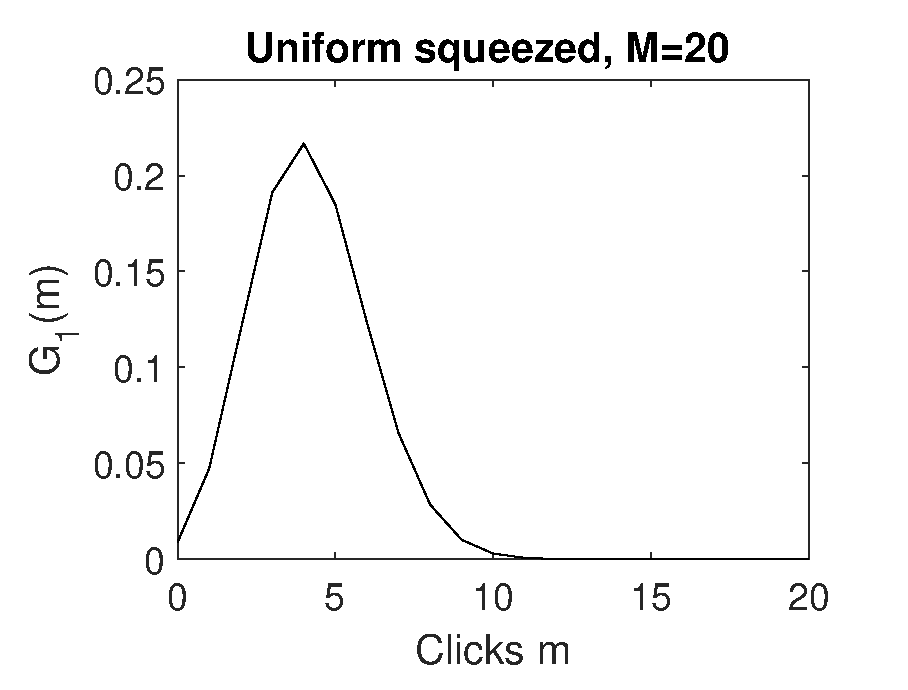
\includegraphics[width=0.5\textwidth]{xQSim_uni_sq_fig}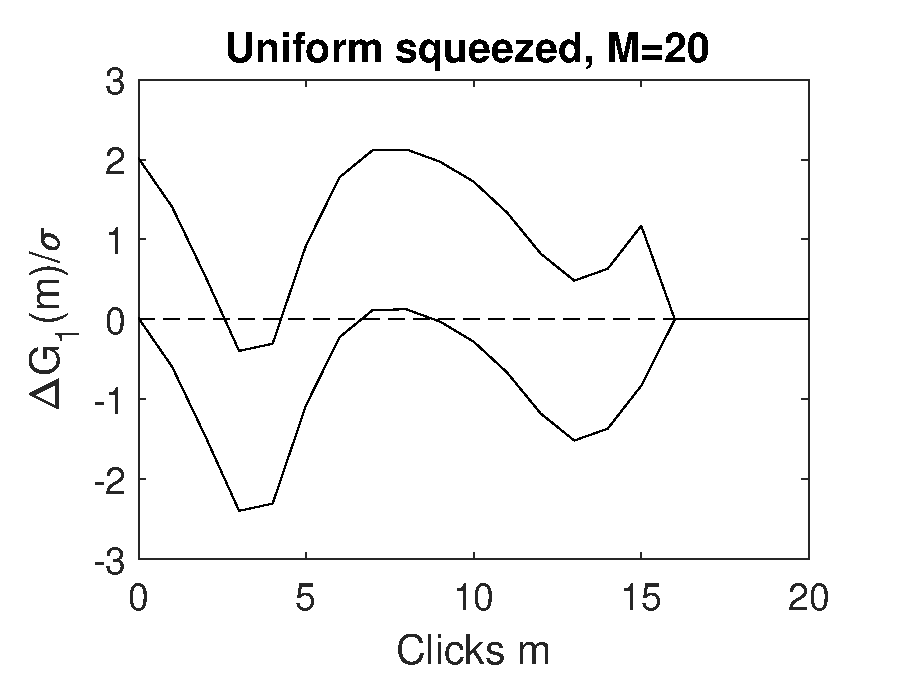
\includegraphics[width=0.5\textwidth]{xQSim_uni_sq_diff_fig}
\par\end{centering}
\caption{Example: $M=20$ mode linear network with uniform squeezed state inputs.
Left graph is simulation versus exact total count probabilities. Right
plot is the normalized difference between simulated (solid line) and
exact (dotted line) distributions. Simulations obtained for $1.2\times10^{6}$
ensembles. }

\end{figure}


\subsubsection{Thermal state}

This example generates total count probabilities for the case of thermal
state inputs with squeezing parameter $\boldsymbol{r}=[1,\dots,1]$
and $\epsilon=1$. The transmission matrix is an $N\times M$ Haar
random unitary with $M=N=100$ and a transmission coefficient of $t=0.5$. 

$\chi^{2}$ statistical test outputs give $\chi^{2}/k\approx1\pm0.4$
for $k=45$ valid bins whilst the $Z$-statistic gives $Z\approx1.5\pm2$. 
\begin{center}
\noindent\doublebox{\begin{minipage}[t]{1\columnwidth - 2\fboxsep - 7.5\fboxrule - 1pt}%
\texttt{}
\begin{lstlisting}
function e1 = xQSim_thermal_test100( )
p.matrix     = @Unitary;
p.M          = 100;
p.N          = 100;
p.name       = sprintf('+P  unitary thermal, M=%d',p.M);
p.t          = 0.5;
p.r          = ones(1,p.M);
p.eps        = ones(1,p.M);
p.Part{1}    = p.M;
p.ensembles  = [1000,100,12];
p.cutoff     = 1.e-7;
p.observe    = {@k1};
p.compare    = {@k1c};
p.glabels    = {{'Clicks m'}};
p.olabels    = {'G_1(m)'};
p.diffplot   = {2};
p.xk{1}      = {0:p.M};
[e1,d,cp]    = xqsim(p);
xgraph(d,cp);
\end{lstlisting}
%
\end{minipage}}
\par\end{center}

~

\begin{figure}[H]
\begin{centering}
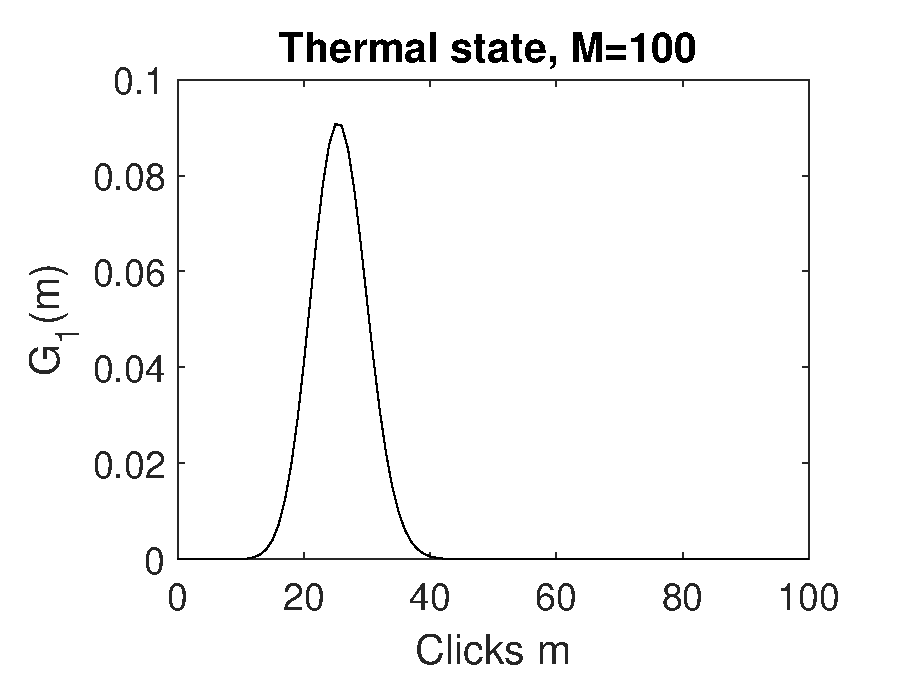
\includegraphics[width=0.5\textwidth]{xQSim_therm_fig}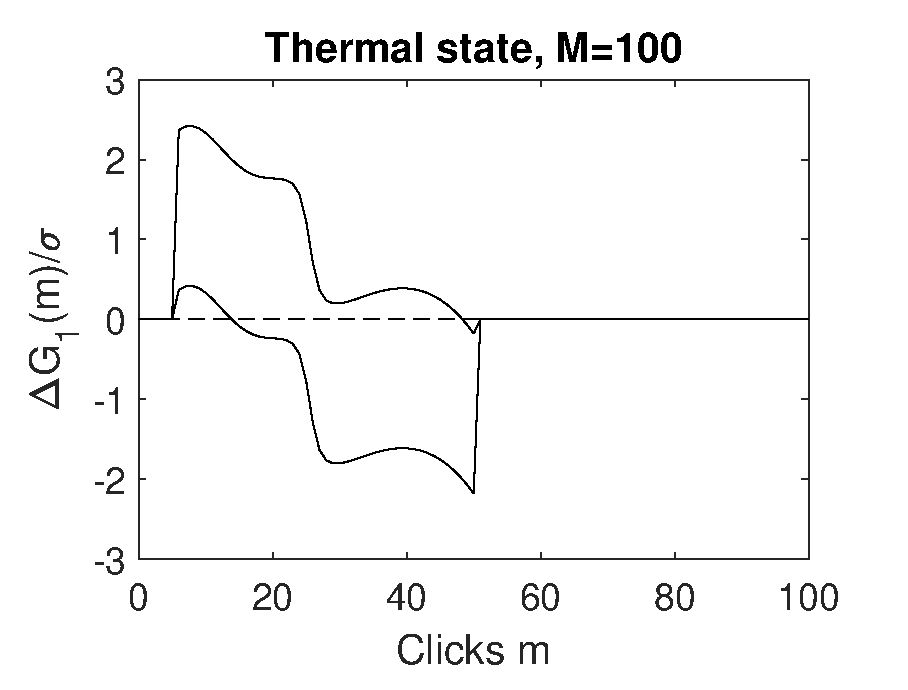
\includegraphics[width=0.5\textwidth]{xQSim_therm_diff_fig}
\par\end{centering}
\caption{Example: $M=100$ mode linear network with thermal state inputs. Left
graph is simulation versus exact total count probabilities. Right
plot is the normalized difference between simulated (solid line) and
exact (dotted line) distributions. Simulations obtained for $1.2\times10^{6}$
ensembles.}
\end{figure}


\subsection{Multidimensional binning}

This example generates output GCPs in two and four dimensions for
the case of non-uniform squeezed inputs. The transmission matrix is
an $N\times M$ identity matrix with $M=N=40$ and a transmission
coefficient of $t=0.5$. 

For simulations with $d>1$, xGraph generates four output plots; two
3D surface plots and two 2D plots. When $d=2$, one surface plot is
the full two-dimensional distribution, whilst the other is the difference
comparison plot. For $d>2$ the surface plots are then two-dimensional
planar slices of, by default, grouped counts $m_{1},m_{2}$ although
this can be changed. Standard 2D plot outputs are always one-dimensional
slices of surface plots. 

Two-dimensional comparisons give $\chi^{2}$ statistical test outputs
of $\chi^{2}/k\approx1\pm0.5$ for $k=169$ valid bins whilst the
$Z$-statistic gives $Z\approx0.7\pm2$. Four-dimensional comparisons
give $\chi^{2}/k\approx1\pm0.5$ for $k=2083$ valid bins and $Z\approx1.4\pm2$.
\begin{center}
\noindent\doublebox{\begin{minipage}[t]{1\columnwidth - 2\fboxsep - 7.5\fboxrule - 1pt}%
\texttt{}
\begin{lstlisting}
function e1 = xQSim_non_uni_sq_test40( )
p.matrix     = @Identity;
p.M          = 40;
p.N          = 40;
p.name       = sprintf('+P non-uniform squeezed, M=%d',p.M);
p.t          = 0.5;
I            = ones(1,p.M/5);
p.r          = [I/4,2*I,4*I,I/2,I];
p.eps        = zeros(1,p.M);
p.Part{1}    = [p.M/2, p.M/2];
p.Part{2}    = [p.M/4, p.M/4,p.M/4,p.M/4];
p.ensembles  = [1000,100,12];
p.cutoff     = 1.e-7;
p.observe    = {@kn,@kn};
p.compare    = {@knc,@knc};
p.glabels    = {{'Clicks m_1','Clicks m_2'},...
     {'Clicks m_1','Clicks m_2','Clicks m_3','Clicks m_4'}};
p.olabels    = {'G_2(m)','G_4(m)'};
p.diffplot   = {2,2};
p.xk{1}      = {0:p.M/2,0:p.M/2};
p.xk{2}      = {0:p.M/4,0:p.M/4,0:p.M/4,0:p.M/4};
[e1,d,cp]    = xqsim(p);
xgraph(d,cp);
\end{lstlisting}
%
\end{minipage}}
\par\end{center}

~

\begin{figure}[H]
\begin{centering}
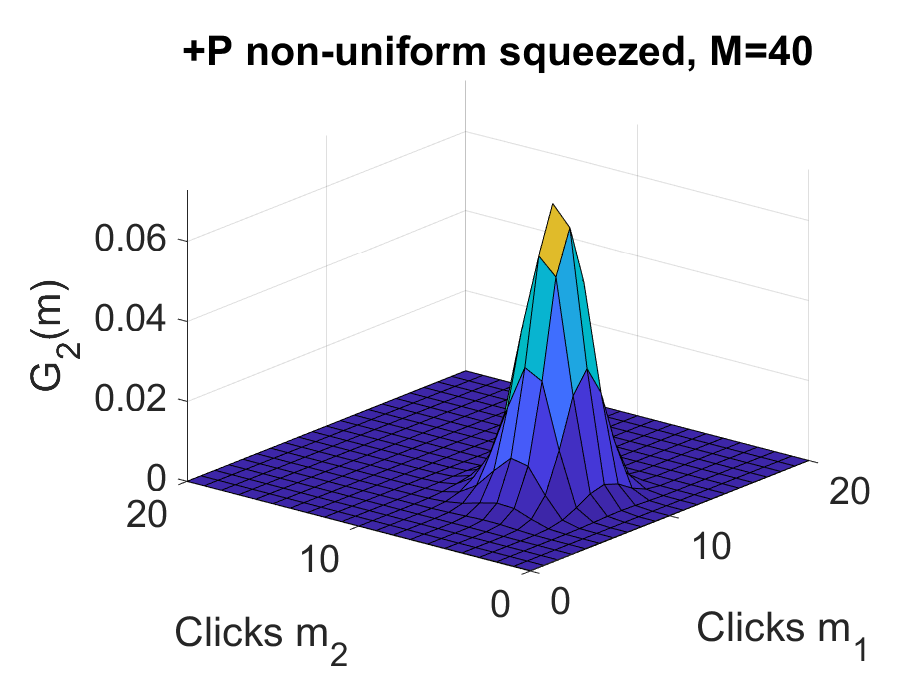
\includegraphics[width=0.5\textwidth]{xQSim_non_uni_sq_2D_fig}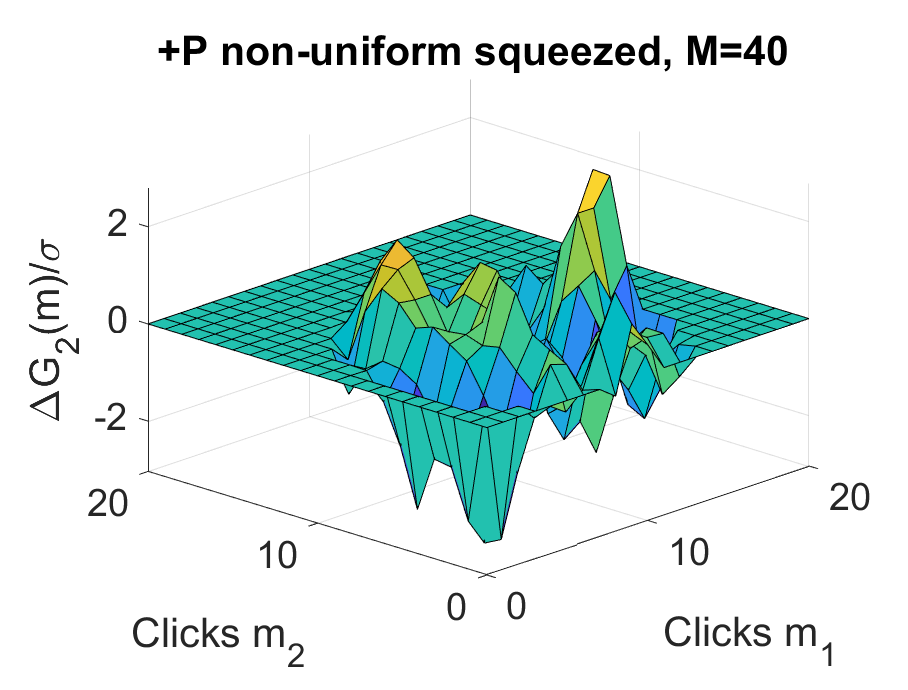
\includegraphics[width=0.5\textwidth]{xQSim_non_uni_sq_2D_diff_fig}
\par\end{centering}
\caption{Example: $M=40$ mode linear network with non-uniform squeezed state
inputs. Left surface plot is simulation versus exact two-dimensional
output probability for all $21^{2}$ data points. Right plot is the
normalized difference between simulated and exact distributions. Simulations
obtained for $1.2\times10^{6}$ ensembles.}
\end{figure}

\begin{figure}[H]
\begin{centering}
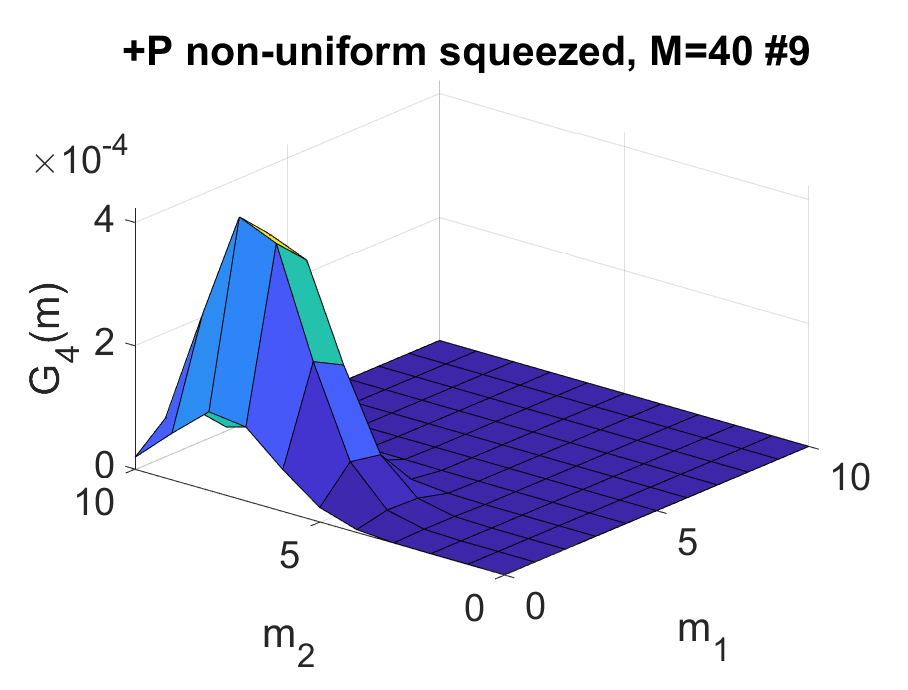
\includegraphics[width=0.5\textwidth]{xQSim_non_uni_sq_4D_fig}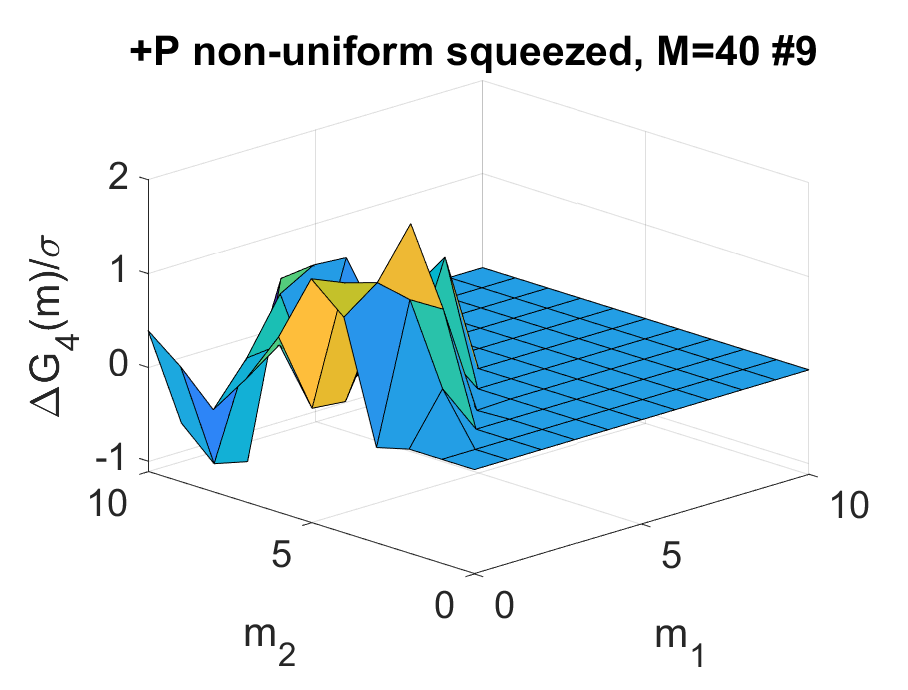
\includegraphics[width=0.5\textwidth]{xQSim_non_uni_sq_4D_diff_fig}
\par\end{centering}
\caption{Example: $M=40$ mode linear network with non-uniform squeezed state
inputs. Left surface plot is a two-dimensional planar slice of simulation
versus exact four-dimensional output probability for $11^{2}$ data
points. Right plot is the normalized difference between simulated
and exact distributions. Simulations obtained for $1.2\times10^{6}$
ensembles.}
\end{figure}


\subsection{Phase-space comparisons}

This example generates intensity correlation moments, $\left\langle \hat{n}'_{1}\dots\hat{n}'_{j}\right\rangle $,
of orders $1\rightarrow5$ for non-uniform thermalized squeezed state
inputs in the positive-P, Wigner and Q phase-space representations
with $\epsilon=0.5$. The transmission matrix is an $N\times M$ identity
matrix with $M=N=20$ and a transmission coefficient of $t=0.5$.

Changing between representations is simple and can be performed on
one script as shown below. However, Wigner and Q representations can
only be used to compute observables with photon number outputs or
quadrature operator moments. 
\begin{center}
\noindent\doublebox{\begin{minipage}[t]{1\columnwidth - 2\fboxsep - 7.5\fboxrule - 1pt}%
\texttt{}
\begin{lstlisting}
function e1 = xQSim_ps_test20( )
p.matrix     = @Identity;
p.M          = 20;
p.N          = 20;
p.name       = sprintf('+P non-uniform thermalized, M=%d',p.M);
p.t          = 0.5;
I            = ones(1,p.M/5);
p.r          = [I/4,2*I,4*I,I/2,I];
p.eps        = 0.5*ones(1,p.M);
p.O{1}       = 1:5;
p.ensembles  = [1000,100,12];
p.cutoff     = 1.e-7;
p.observe    = {@nm};
p.compare    = {@nmc};
p.glabels    = {{'Order'}};
p.olabels    = {'<n_1...n_j>'};
p.diffplot   = {2};
p.xk{1}      = p.O(4);

pW          = p;
pW.method   = 2;
pW.name     = sprintf('W non-uniform thermalized, M=%d',p.M);

pQ          = p;
pQ.method   = 3;
pQ.name     = sprintf('Q non-uniform thermalized, M=%d',p.M);

[e1,d,cp]    = xqsim({p,pW,pQ});
xgraph(d,cp);
\end{lstlisting}
%
\end{minipage}}
\par\end{center}

~

\begin{figure}[H]
\begin{centering}
\includegraphics[width=0.5\textwidth]{xQSim_non_uni_th_+P_fig}
\par\end{centering}
\begin{centering}
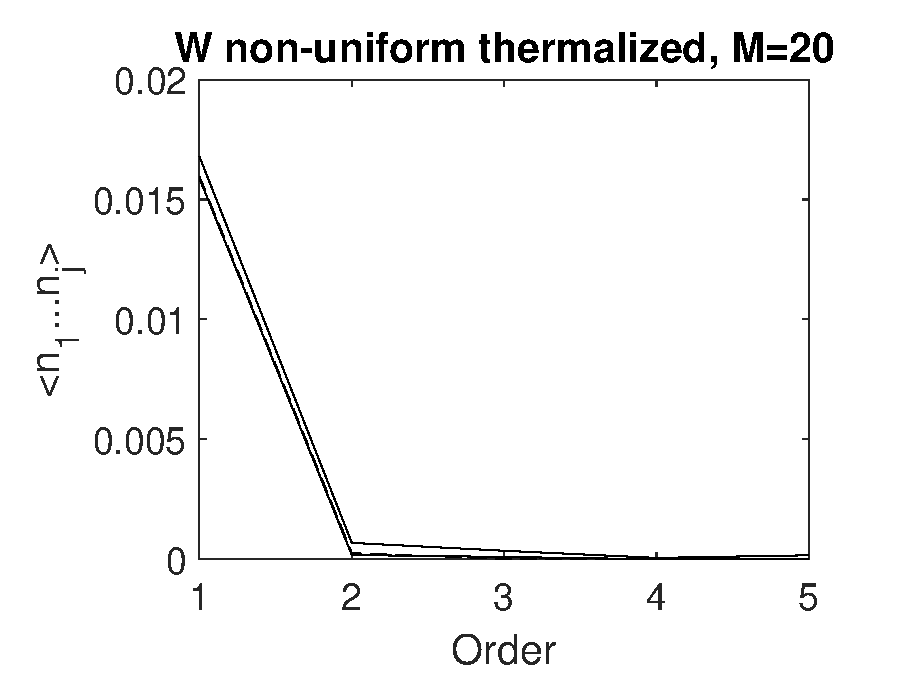
\includegraphics[width=0.5\columnwidth]{xQSim_non_uni_th_W_fig}
\par\end{centering}
\centering{}\includegraphics[width=0.5\textwidth]{xQSim_non_uni_th_Q_fig}\caption{Example: Intensity correlation moments versus correlation order. Simulations
are denoted by the solid line and use the positive-P (top), Wigner
(middle) and Q (bottom) representations whilst the dashed lines denotes
exactly computed correlation moments. While the normally ordered positive-P
probabilities agree with the exact calculations, the Wigner and Q
representations deviate significantly from exact calculations which
increase with correlation order. This deviation is due to vacuum fluctuations
causing sampling errors increasing with correlation order. }
\end{figure}


\subsection{Experimental examples}

This subsection contains examples for simulations using experimental
data from the $100$-mode implementation of Zhong et al \cite{Raw100,zhong2020quantum}.
Although multiple examples are given in the \textit{xQSimExamples}
folder, we focus on generating comparisons of higher-order click correlations
and random permutations of binary patterns in this manual. 

\subsubsection{High-order correlations}

This example generates comparisons of click correlation moments of
first and second order which are defined as 

\[
\left\langle \hat{\pi}_{j}(1)\right\rangle 
\]

\[
\left\langle \hat{\pi}_{j}(1)\hat{\pi}_{k}(1)\right\rangle .
\]

Comparisons can be obtained for all possible combinations of output
modes, which follows the binomial coefficient $\binom{M}{n}$, or
for a subset of these combinations. The subset comparisons are preferable
for graphing, whilst the full comparison of output modes is preferable
for statistical tests to ensure all possible correlations are observed.
Not observing all correlations will alter the statistical test outputs
as there are fewer valid bins. 

Inputs are thermalized squeezed states with decoherence coefficient
$eps=0.0932$ and transmission $t=1.0235$. Simulations were performed
for $1.44\times10^{7}$ ensembles. First-order correlations have statistical
test outputs of $\chi^{2}/k\approx5.25\times10^{3}$ and $Z\approx347$,
for $k=100$, whilst second-order marginals give $\chi^{2}/k\approx4.99\times10^{3}$
and $Z\approx2.4\times10^{3}$, for $k=4950$. 
\begin{center}
\noindent\doublebox{\begin{minipage}[t]{1\columnwidth - 2\fboxsep - 7.5\fboxrule - 1pt}%
\texttt{}
\begin{lstlisting}
function e = xQSim_experiment_HOC( )
p.name      = 'Click correlation,M=100'
p.matrix    = @expmatrix;
p.M         = 100;
p.N         = 50;
p.r         = @expsqueeze;
p.CO{2}     = 2;
p.CO{3}     = 2;
p.ensembles = [6000,200,12];
p.t         = 1.0235;
p.eps       = 0.0932;
p.counts    = 51392341;
p.mincount  = 10;
p.cutoff    = 1e-7;
p.observe   = {@k,@kmsub,@km2};
p.compare   = {@expk,@expk2ms,@expk2m};
p.diffplot  = {2,2,2};
p.glabels   = {{'j'},{'j,k'}{'j<k'}};
p.olabels   = {'<\pi_j(1)>','G^{(2)}','<\pi_j(1)\pi_k(1)>'};
p.xk{2}     = {0:p.M-1};
p.xk{3}     = {0:4950};
[e,d,cp]    = xqsim(p);
xgraph(d,cp);
\end{lstlisting}
%
\end{minipage}}
\par\end{center}

~

\begin{figure}[H]
\begin{centering}
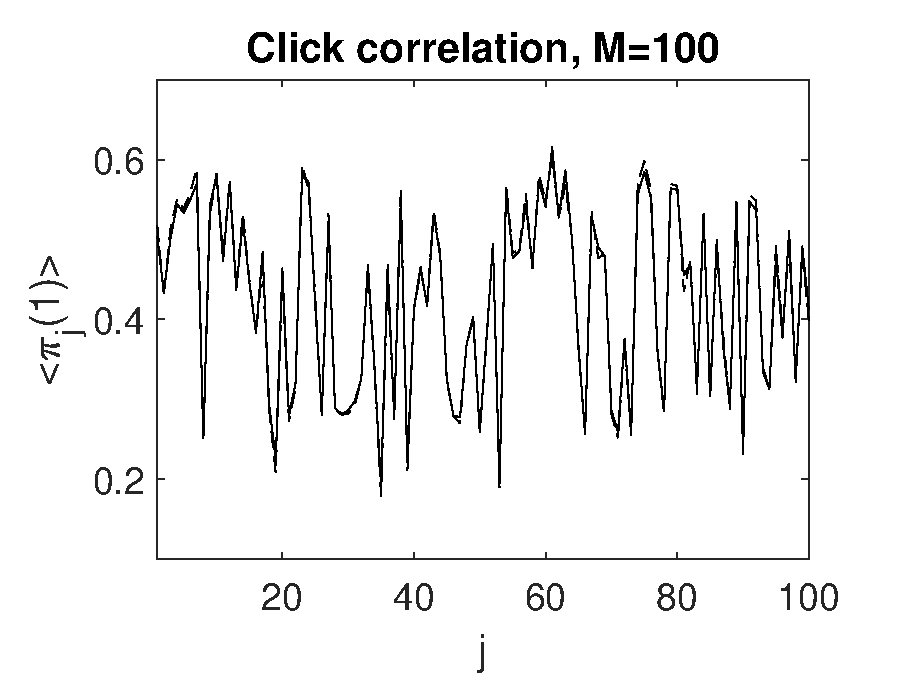
\includegraphics[width=0.5\textwidth]{xQSim_exp_FO_fig}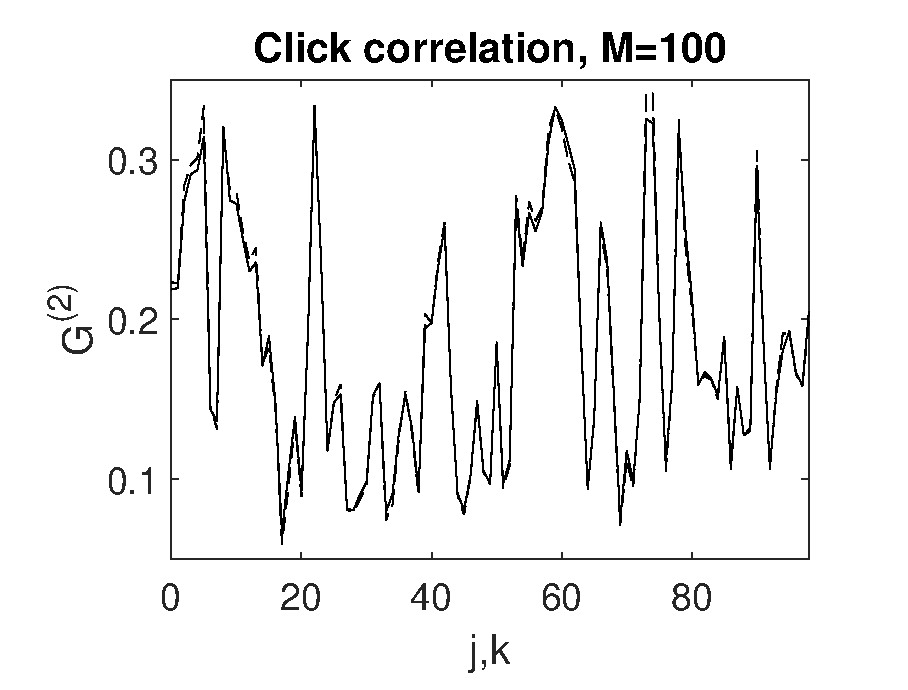
\includegraphics[width=0.5\textwidth]{xQSim_exp_SO_fig}
\par\end{centering}
\caption{Example: Comparisons of click correlations of experiment (dashed line)
versus theory (solid line). The left graph plots correlations of first-order
for all possible combinations of output modes. Right graph contains
only the first $99$ second-order correlations for graphical simplicity. }
\end{figure}


\subsubsection{Random permutations}

This example generates comparisons of two-dimensional GCPs for binary
patterns that have been randomly permuted. Inputs are thermalized
squeezed states with decoherence coefficient $eps=0.0932$ and transmission
$t=1.0235$. Data for three random permutations from this experiment
are available in the folder \textit{xQSimGBSExperiments}, however
more can be readily obtained. 

Permutations are input through the parameter \textit{p.permute}, which
is assumed to be a $1\times M$ row vector, and are applied to the
transmission matrix, changing the row order according to the mode
ordering of the permutation. User's can either manually permute output
modes, e.g. $p.permute=[15,8,44,\dots]$, or use permutations generated
from data extraction algorithms which are loaded from relevant .mat
files by the function \textit{xqpermutation} (see subsection. \ref{subsec:Data-extraction}).
Note, manual permutation vectors are only applied to the transmission
matrix rows, not the binary data which must be permuted before being
binned. 

Simulations can then be performed, with total count and click correlations
unaffected by the permutation. Since each permutation produces comparisons
of different correlations, each test will output different $\chi^{2}$
and $Z$-statistic results as well as normalized difference graphs.
An example of this is given in the below figure. 
\begin{center}
\noindent\doublebox{\begin{minipage}[t]{1\columnwidth - 2\fboxsep - 7.5\fboxrule - 1pt}%
\texttt{}
\begin{lstlisting}
function e = xQSim_experiment_permute( )
p.name      = 'Random permutation 1'
p.matrix    = @expmatrix;
p.M         = 100;
p.N         = 50;
p.r         = @expsqueeze;
p.Part{3}   = [50, 50];
p.Part{4}   = [25,25,25,25];
p.ensembles = [5000,20,12];
p.t         = 1.0235;
p.eps       = 0.0932;
p.counts    = 51392341;
p.mincount  = 10;
p.cutoff    = 1e-7;
p.permute   = xqpermutation;
p.observe   = {@k,@k1,@kn};
p.compare   = {@expk,@expk1,@expk2};
p.logs{2}   = [0,1];
p.logs{3}   = [0,0,1];
p.diffplot  = {2,2,2};
p.glabels   = {{'j'},{'m'},{'Clicks m_1','Clicks m_2'}};
p.olabels   = {'<\pi_j(1)>','G_1(m)','G_2(m)'};
p.xk{2}     = {0:p.M};
p.xk{3}     = {0:50,0:50};
[e,d,cp]    = xqsim(p);
xgraph(d,cp);
\end{lstlisting}
%
\end{minipage}}
\par\end{center}

~

\begin{figure}[H]
\begin{centering}
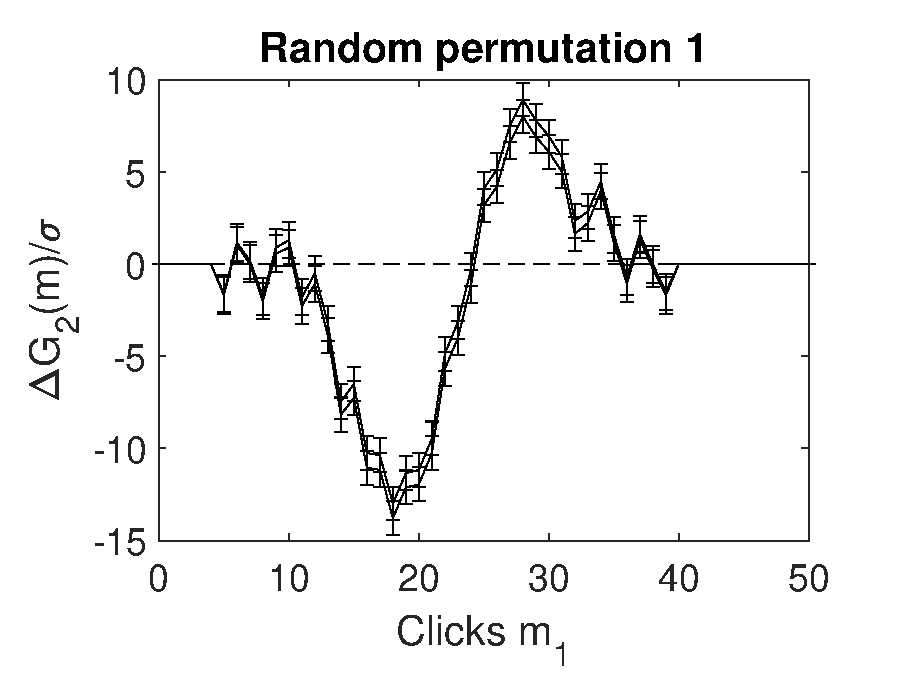
\includegraphics[width=0.5\textwidth]{xQSim_exp_rand_p1}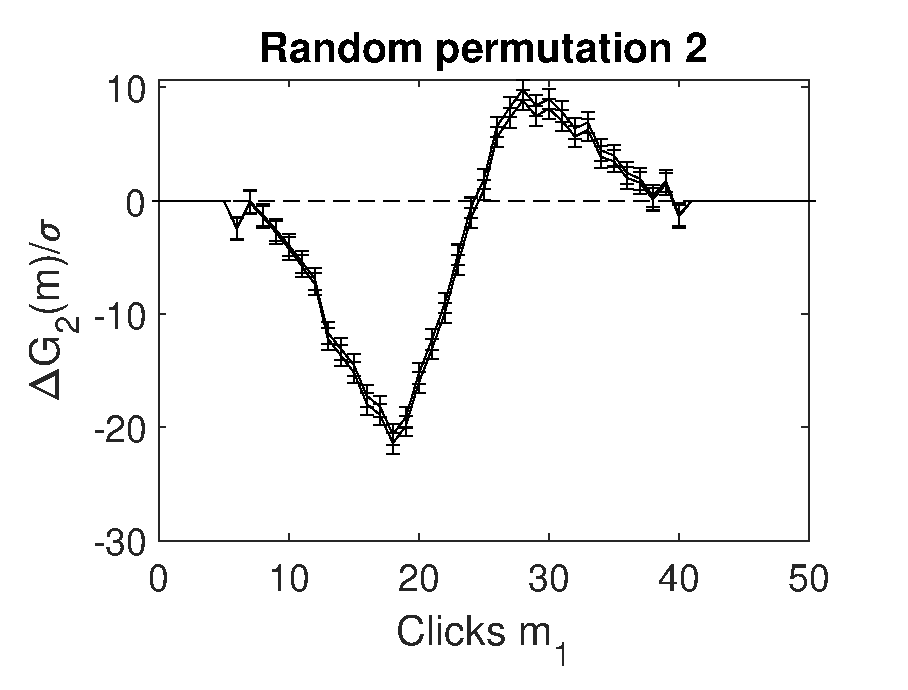
\includegraphics[width=0.5\textwidth]{xQSim_exp_rand_p2}
\par\end{centering}
\caption{Example: Normalized difference of theory versus experiment of two-dimensional
binning from two separate random permutations. Left graph is a one-dimensional
slice of the full distribution with statistical test outputs of $\chi^{2}/k\approx28$
for $k=973$ and $Z\approx134$. Right graph is also a one-dimensional
slice of the full distribution with a different random permutation
applied. Statistical test outputs are $\chi^{2}/k\approx47$ for $k=976$
and $Z\approx173$ for this permutation. Both simulations were performed
for $1.2\times10^{6}$ ensembles. }

\end{figure}


\section{xQSim reference \label{sec:xqSIM-reference}}

\textbf{\emph{This section gives a reference guide to the xQSim parameters
and functions.}}

\subsection{Included programs}

The package provided has six parts:
\begin{enumerate}
\item \textbf{xQSimCode. }This contains all the main quantum simulation
codes, from observable and comparison functions to quantum phase-space
sample generating functions. 
\item \textbf{xQSimExamples. }This has the scripts used to simulate experiments
for comparisons, as well as scripts used for testing.
\item \textbf{xQSimData. }This has scripts used for simulating data from
recent Gaussian boson sampling experiments.
\item \textbf{xQSimDocumentation. }This provides the documentation, including
this report and a separate manual for the graphics program \textit{xGraph}.
\item \textbf{xGraph. }This contains a multidimensional graphics program
which is also used in the stochastic differential equation software
package \textit{xSPDE}. 
\item \textbf{xQSimGBSExperiments. }This has recent public experimental
data from Refs. \cite{zhong2020quantum,Zhong2021Phase}, and data
extraction codes for reference purposes.
\end{enumerate}

\subsection{xQSim function call}

The simulation function takes an input of parameter structures that
define a sequence of networks. Each network in the sequence can be
repeated, with recycling of the amplitudes, which are then combined
with new squeezed or coherent inputs. Any input parameters or functions
that are omitted are given appropriate default values.

Simulations carried out by the code are performed by other specialized
internal functions. Input parameters come from an \textbf{input} cell
array of structures, while output is saved in a \textbf{data} array,
and optionally in a file. During the simulation, global averages and
error-bars are calculated for sampling errors. When completed, timing
and errors are printed.

The \emph{xQSim} function call syntax is: \emph{{[}error,data,output{]}
= xQSim(input);}

The input data includes parameters and methods, but with an open architecture
for extensibility. Most functions are modular and replaceable. This
is as easy as defining a new function handle to replace the default
value. The code folder includes examples of how these are written.
All output observables are divided up into a cell array of data graphs,
generated in parallel.

To explain this in full detail, 
\begin{itemize}
\item Simulation parameters are stored in the \textbf{\emph{input}} cell
array. 
\item This describes a sequence of parameter structures, so that \textbf{\emph{input=\{p1,p2,...\}}}. 
\item Each structure \textbf{\emph{p1,p2,..}}\textbf{.} generates an output
which is the input of the next. 
\item The main simulation function is called using \textbf{\emph{xQSim(input).}} 
\item The errors and integration time are returned in the \textbf{\emph{error}}\textbf{
}vector 
\item Averages are recorded sequentially in the \textbf{\emph{data}} cell
array. 
\item Parameters including defaults are returned in the \textbf{\emph{output}}
cell array. 
\end{itemize}
The sequence \emph{input} defines a sequence of individual simulations,
with parameters that specify the simulation functions and give the
equations and observables. If there is only one simulation, just one
data structure is needed, without a cell array. In addition, xQSim
can generates graphs with a companion graphics program, xGraph.

\subsection{Parameters and functions}

The xQSim input objects include parameters and functions. Many xQSim
functions are modular and replaceable, through defining a new function
handle to replace the default value.

There are standard conventions used throughout: 
\begin{itemize}
\item All arguments in square brackets are optional, but may be needed only
in specific cases. 
\item The last argument, \emph{p,} is the parameter structure. 
\end{itemize}
The user-definable functions, input and output field dimensions and
calling arguments are:\\

\begin{center}
\begin{tabular}{|c|c|c|}
\hline 
Label & Arguments & Output dimensions\tabularnewline
\hline 
\hline 
\emph{a=qgen} & \emph{(a,p): $a=(2M\times S_{1})$,~~~p={[}struct{]}} & \emph{$a=(2M\times S_{1})$}\tabularnewline
\hline 
\emph{permute=xqpermutation} & \textasciitilde{} & Arbitrary: $1\times M$\tabularnewline
\hline 
\emph{o=observe\{n\}} & \emph{(a,p): $a=(2M\times S_{1})$,~~~p={[}struct{]}} & Arbitrary: $m_{1}\times m_{2}\ldots\times m_{n}$\tabularnewline
\hline 
\emph{c=compare\{n\}} & \emph{$(p)$,~~~p={[}struct{]}} & Match observe: $m_{1}\times m_{2}\ldots\times m_{n}$\tabularnewline
\hline 
\end{tabular}\\
\par\end{center}

Notes 
\begin{itemize}
\item \textbf{\emph{qgen}}\textbf{ has a default, namely $xqgen$, which
can be user modified}
\item \textbf{qgen input amplitudes are used for recycling. If this is not
required, just use $(\sim,p):$}
\item \textbf{data outputs to xGraph include two extra dimensions, $m_{l}\times m_{1}\times m_{2}\ldots\times m_{n}\times m_{e}$}
\item \textbf{The first graphics $m_{l}$ dimension is reserved for plotting
multiple lines on graphs}
\item \textbf{Obtaining multiple lines requires modifying the output data
file before xGraph}
\item \textbf{The $m_{e}$ dimension is used for error bars. Here $m_{e}=3$
stores the sampling error bars}
\end{itemize}

\subsection{Customization guide}

To define your own stochastic generation function, include in the
input the line:

\begin{center}
\noindent\doublebox{\begin{minipage}[t]{1\columnwidth - 2\fboxsep - 7.5\fboxrule - 1pt}%
\texttt{p.gen=@Mygen;}%
\end{minipage}}
\par\end{center}

Next, include anywhere on your Matlab path the function definition,
for example:

\begin{center}
\noindent\doublebox{\begin{minipage}[t]{1\columnwidth - 2\fboxsep - 7.5\fboxrule - 1pt}%
\texttt{function a = Mygen(a,p)}

\texttt{\% a = Mygen(a,p) generates stochastic variables my way!}

\texttt{..}

\texttt{a = ...;}

\texttt{end}%
\end{minipage}}
\par\end{center}

~\\
Similarly, to define your own observe function for (say) data graph
$6$, include in the input the line:

\begin{center}
\noindent\doublebox{\begin{minipage}[t]{1\columnwidth - 2\fboxsep - 7.5\fboxrule - 1pt}%
\texttt{p.observe\{6\}=@Myobserve;}%
\end{minipage}}
\par\end{center}

Next, include anywhere on your Matlab path the function definition,
for example:

\begin{center}
\noindent\doublebox{\begin{minipage}[t]{1\columnwidth - 2\fboxsep - 7.5\fboxrule - 1pt}%
\texttt{function d = Myobserve(a,p)}

\texttt{\% d = Myobserve(a,p) generates observables my way!}

\texttt{..}

\texttt{d = ...;}

\texttt{end}%
\end{minipage}}
\par\end{center}

~\\
To define your own comparison function for the same graph, include
in the input the line:

\begin{center}
\noindent\doublebox{\begin{minipage}[t]{1\columnwidth - 2\fboxsep - 7.5\fboxrule - 1pt}%
\texttt{p.compare\{6\} = @Mycompare;}%
\end{minipage}}
\par\end{center}

Next, include anywhere on your Matlab path the compare definition,
for example:

\begin{center}
\noindent\doublebox{\begin{minipage}[t]{1\columnwidth - 2\fboxsep - 7.5\fboxrule - 1pt}%
\texttt{function c = Mycompare(a,p)}

\texttt{\% c = Mycompare(a,p) generates comparisons my way!}

\texttt{..}

\texttt{c = ...;}

\texttt{end}%
\end{minipage}}
\par\end{center}

\subsection{Hints}
\begin{itemize}
\item When using xQSim, it is a good idea to first run the batch test script,
xQSimtest.m. 
\item xQSimtest.m tests your parallel toolbox installation. If you have
no license for this, omit the third ensemble setting.
\item To create a script, it is often easiest to start with an existing
script with similar requirements: see Examples folder.
\item Graphics parameters can also be included in the parameter structure
$\mathbf{p}$, either before or after calling $qcpsim$, to modify
graphs.
\item Comparison functions can be included to compare with analytic or experimental
results.
\item A full list of functionality is listed below.
\end{itemize}
The input data, here labeled $input$, is a sequence of parameter
structures that are labeled $p$. All of the input parameters and
data are later passed to the $xgraph$ function. The input data can
be numbers, vectors, strings, functions and cell arrays. These are
lists of data enclosed in curly brackets, $\{\}$. All xQSim metadata
has preferred values, so only changes from the preferences need to
be input. The resulting combined input including preferred values,
is stored internally as a sequence of structures in a cell array to
describe the simulation sequence.

Simulation metadata, including all preferred default values that were
used in a particular simulation, is also stored in the xQSim output
files. This is done in the Matlab $.mat$ format, for simplicity so
the entire simulation can be easily reconstructed or changed. 

Some conventions are used to simplify inputs, as follows: 
\begin{itemize}
\item \textbf{Most input data has default values}
\item \textbf{Vector inputs of numbers are enclosed in square brackets,
{[}...{]}. }
\item \textbf{Where multiple inputs of strings, functions or vectors are
needed they should be enclosed in curly brackets, \{...\}, to create
a cell array. }
\item \textbf{Vector or cell array inputs with only one member don't require
brackets. }
\item \textbf{Incomplete vector or array inputs are completed with the last
default or input value.}
\item \textbf{Default parameters are checked by inspecting the outputs,
or setting verbose = 2.}
\end{itemize}
In the output data arrays, the last index has $m_{e}=1$ for the averages.
The first error field, $m_{e}=2$, is reserved for any systematic
errors like step-sizes. The last error field, $m_{e}=3$ is used for
storing one standard deviation error-bar estimates due to computational
sampling errors.

\subsection{Parameter table\label{sec:Simulation-parameters}}

Simulation parameters are stored in a parameter structure which is
passed to the $xsim$ program. Inputs have default values, which are
user-modifiable through the\emph{ xpreferences} function. Defaults
can be checked by including the input $verbose=2$\emph{.} All the
inputs are part of a structure passed to xQSim. If a cell array of
multiple structures are input, these are executed in sequence, with
the output of the first simulation passed to the second, then the
third, and so on.

\begin{center}
\begin{tabular}{|c|c|c|c|}
\hline 
Label & Type & Default & Description\tabularnewline
\hline 
\hline 
\textit{deco} & string & '' & Decoherence factors used for optimization\tabularnewline
\hline 
\textit{bits} & integer & None & Number of bits used for data extraction\tabularnewline
\hline 
CO & integer & None & Correlation order\tabularnewline
\hline 
\emph{compare} & function handles & {[}{]} & Optional comparison functions\tabularnewline
\hline 
\emph{counts} & integer & 0 & Total experimental counts for $\chi^{2}$ tests\tabularnewline
\hline 
\emph{cutoff} & real & -1.e100 & Lower cutoff for graphs and $\chi^{2}$\tabularnewline
\hline 
\emph{cyc} & integer & 1 & Number of cycles of the network\tabularnewline
\hline 
\emph{ensembles} & vector & {[}1,1,1{]} & Size of vector, serial, parallel ensemble\tabularnewline
\hline 
\emph{eps} & vector & 0 & An n-dimensional decoherence factor\tabularnewline
\hline 
M & integer & 1 & Total matrix size\tabularnewline
\hline 
\emph{matrix} & matrix function & Identity & An $M\times M$ transfer matrix function\tabularnewline
\hline 
\emph{method} & integer & 1 & Phase-space method: $m=1,2,3$\tabularnewline
\hline 
\emph{mincount} & integer & 0 & Minimum count for $\chi^{2}$ tests\tabularnewline
\hline 
N & integer & 1 & Number of excited input modes\tabularnewline
\hline 
\emph{name} & character & '' & Name of simulation\tabularnewline
\hline 
O & vector & None & Vector of various correlation orders\tabularnewline
\hline 
\emph{observe} & function handles & $\{@(a,p)\,a\}$ & Observable functions\tabularnewline
\hline 
\emph{permute} & integer vector & $[1,2,3,\dots,M]$ & Random permutation of outputs\tabularnewline
\hline 
\emph{pnames} & array of characters & \{'+P ','W ','Q '\} & Names of phase-space methods\tabularnewline
\hline 
\emph{qgen} & function handle & $@xqgen$ & Stochastic generation code\tabularnewline
\hline 
\emph{r} & vector or function & 0 & An n-dimensional squeezing vector\tabularnewline
\hline 
re & vector & 1 & An n-dimensional recycling factor\tabularnewline
\hline 
\emph{t} & vector & 1 & An n-dimensional transmission factor\tabularnewline
\hline 
\emph{Tname} & unitary name & matrix(0) & Name of transmission matrix\tabularnewline
\hline 
\emph{verbose} & integer & 0 & Flag for printing verbosity level: 0,1,2\tabularnewline
\hline 
\end{tabular}
\par\end{center}

\subsection{Parameter reference}

The following parameters can be applied to each member of the simulation
sequence. For single-input, single-pass GBS experiments, they are
only specified once.

\subsubsection{bits}
\begin{description}
\item [{Default:}] None
\end{description}
Integer used to define the bit-type encoding of experimental binary
data files. Only used for integrated data extraction codes. 
\begin{itemize}
\item p.bits 
\end{itemize}

\subsubsection{compare}
\begin{description}
\item [{Default:}] {[}{]}
\end{description}
Cell array of function handles to generate the comparison data. A
large number of functions equivalent to common hermitian operators
are available for analytically known cases..
\begin{itemize}
\item p.compare = \{@function,..\}
\end{itemize}

\subsubsection{CO}
\begin{description}
\item [{Default:}] None
\end{description}
Used to define the correlation order for calculating click correlation
moments or marginal probabilities of output distribution. 
\begin{itemize}
\item $p.CO$
\end{itemize}

\subsubsection{counts}
\begin{description}
\item [{Default:}] 0
\end{description}
Used to define the total counts for calculating count numbers and
minimum count cutoffs when there is experimental data on experimental
count probabilities.
\begin{itemize}
\item $p.counts>0$
\end{itemize}

\subsubsection{cutoff}
\begin{description}
\item [{Default:}] -1E-100
\end{description}
Used to define a lower cutoff, especially for probability data, where
a small positive value, e.g. $10^{-7}$, should be used. This is useful
for log graphs and $\chi^{2}$ fits. 
\begin{itemize}
\item $p.cutoff$
\end{itemize}

\subsubsection{cyc}
\begin{description}
\item [{Default:}] 1
\end{description}
Number of cycles of the network simulated.
\begin{itemize}
\item p.cyc >0
\end{itemize}

\subsubsection{deco}
\begin{description}
\item [{Default:}] ' '
\end{description}
String used to output deocherence factors $eps$ and $t$ during optimization.
Only needs to be used if Matlabs \textit{fminsearch} is performing
optimization. 
\begin{itemize}
\item p.deco 
\end{itemize}

\subsubsection{ensembles}
\begin{description}
\item [{Default:}] {[}1,1,1{]}
\end{description}
Number of ensembles used in simulations. The first is the local vector
ensemble. The second is the number of serial repeats. The third is
the number or parallel repeats. Note that serial and parallel repeats
are used for sampling error estimation.
\begin{itemize}
\item p.name = {[}ens1,ens2,ens3{]}
\end{itemize}

\subsubsection{eps}
\begin{description}
\item [{Default:}] 0
\end{description}
This gives a real decoherence vector that is input. It is expected
to be of length at least $p.N$. If smaller, it will be expanded to
length $p.N$. The values should such that $0\le p.eps\le1$.
\begin{itemize}
\item p.eps 
\end{itemize}

\subsubsection{M}
\begin{description}
\item [{Default:}] 1
\end{description}
Total number of input and/or output modes to the network.
\begin{itemize}
\item p.M >0
\end{itemize}

\subsubsection{matrix}
\begin{description}
\item [{Default:}] @Identity
\end{description}
Function handle to generate the linear network matrix. Both Identity
and random Unitary matrices are supplied. It can also be just an $M\times M$
complex matrix, for small test matrices entered inline.
\begin{itemize}
\item p.matrix = @function
\end{itemize}

\subsubsection{method}
\begin{description}
\item [{Default:}] 1
\end{description}
The phase-space method, where 1 = generalized P-representation, 2
= Wigner representation, 3 = Husimi (Q) representation
\begin{itemize}
\item p.method > 0
\end{itemize}

\subsubsection{mincount}
\begin{description}
\item [{Default:}] 0
\end{description}
Used to set a lower bound on calculations for chi-square fits, when
there is experimental data on experimental count probabilities. A
typical value here is $10$.
\begin{itemize}
\item $p.mincount>0$
\end{itemize}

\subsubsection{N}
\begin{description}
\item [{Default:}] 1
\end{description}
Number of input modes excited, less than or equal $M$
\begin{itemize}
\item p.N >0
\item p.M >0
\end{itemize}

\subsubsection{name}
\begin{description}
\item [{Default:}] ' '
\end{description}
Name used to label simulation, usually corresponding to the equation
or problem solved, and will be passed to the xGraph program if it
is used.
\begin{itemize}
\item p.name = 'your project name'
\end{itemize}

\subsubsection{O}
\begin{description}
\item [{Default:}] None
\end{description}
Used to define a vector of correlation orders to simulate mean click
or photon number correlations over adjacent channels. 
\begin{itemize}
\item $p.O$
\end{itemize}

\subsubsection{observe}
\begin{description}
\item [{Default:}] \{@(a,p) mean(real(a),2)\}
\end{description}
Cell array of function handles to generate the observable phase-space
averages. A large number of functions equivalent to commonly used
hermitian operators are available.
\begin{itemize}
\item p.observe = \{@function,..\}
\end{itemize}

\subsubsection{permute}
\begin{description}
\item [{Default:}] $[1,2,3,\dots,M]$
\end{description}
Random permutation vector of size $1\times M$ obtained either manually
or via a data extraction output which is applied to rows of the transmission
matrix for phase-space simulations. 
\begin{itemize}
\item p.permute = xqpermutation
\end{itemize}

\subsubsection{pnames}
\begin{description}
\item [{Default:}] \{\textquoteright +P \textquoteright ,\textquoteright W
\textquoteright ,\textquoteright Q \textquoteright\}
\end{description}
Cell vector of names used to label the phase-space representation,
to allow future expansion or changes. Normally is not changed from
default and can be omitted.
\begin{itemize}
\item p.pnames = \{'your favorite method'\}
\end{itemize}

\subsubsection{qgen}
\begin{description}
\item [{Default:}] @qgen
\end{description}
Name of network quantum noise function. The default qgen function
is used for GBS, and in this case, just omit $qgen$.
\begin{itemize}
\item p.qgen = @yourgenerator
\end{itemize}

\subsubsection{r}
\begin{description}
\item [{Default:}] 0
\end{description}
This gives a real squeezing vector that is input. It is expected to
be of length at least $p.N$. If smaller, it will be expanded to length
$p.N$. The entries with index greater than $p.N$ are set to zero.
Can be replaced by a function call for large quantities of data.
\begin{itemize}
\item p.r 
\end{itemize}

\subsubsection{re}
\begin{description}
\item [{Default:}] 0
\end{description}
This gives a real recycling amplitude. It is expected to be of length
$p.M$. If smaller, it will be expanded to length $p.M$. The entries
with index greater than $p.M$ are set to zero. This allows previous
amplitudes to be recycled.
\begin{itemize}
\item $p.re\le1$ 
\end{itemize}

\subsubsection{t}
\begin{description}
\item [{Default:}] 1
\end{description}
This gives a real transmission vector that is input. It is expected
to be of length $p.M$. If smaller, it will be expanded to length
$p.M$. The entries with index greater than $p.M$ are set to zero.
This allows corrections to be made to the measured transmission matrix.
\begin{itemize}
\item $p.t\le1$ 
\end{itemize}

\subsubsection{Tname}
\begin{description}
\item [{Default:}] matrix(0)
\end{description}
Name used to label type of network matrix. Usually it is returned
by the matrix function to give the default name. However, other matrix
names can be entered here.
\begin{itemize}
\item p.Tname = 'your transmission matrix name'
\end{itemize}

\subsubsection{verbose}
\begin{description}
\item [{Default:}] 0
\end{description}
Print flag for output information while running xQSim. If ``verbose
= 0``, most output is suppressed, while ``verbose = 1`` displays a
progress report, and ``verbose = 2`` also generates a readable summary
of the parameters as a record.
\begin{itemize}
\item p.verbose >= 0
\end{itemize}

\section{xGraph reference\label{sec:xGRAPH-reference}}

The graphics function provided is a general purpose multidimensional
batch graphics code, xGraph, which can be called when xQSim is finished.
The results are graphed and output if required. Alternatively, xGraph
can be replaced by another graphics code, or it can be used to process
the data generated by xQSim at a later time.

The program is described elsewhere, but the documentation is replicated
here for users who wish to use it. The \emph{xGraph} function call
syntax is: 
\begin{itemize}
\item \textbf{\emph{xgraph (data {[},input{]})}} 
\end{itemize}
This takes simulation \emph{data} and \emph{input} cell arrays with
graphics parameters, then plots graphs. The \emph{data} should have
as many cells as there are \emph{input} cells, for sequences. The
data can include comparisons, either analytic or experimental, and
error-bars for both the simulations and the comparisons, since either
may have sampling or other errors.

If \emph{data = 'filename.h5'} or\emph{ 'filename.mat'}, the specified
file is read both for \emph{input} and \emph{data}. Here \emph{.h5}
indicates an HDF5 file, and \emph{.mat} indicates a Matlab file.

When the \emph{data} input is a filename, parameters in the file can
be replaced by new \emph{input} parameters that are specified. Any
stored \emph{input} parameters in the file are overwritten when graphs
are generated. This allows graphs of data to be modified retrospectively,
if the simulation takes too long to be run again in a reasonable timeframe.

\subsection{Parameter and data structures}

This is a batch graphics function, intended to process quantities
of graphics data in sequence, input as a cell array of multi-dimensional
data. Theoretical and/or experimental data is passed to the graphics
program, including the complete \emph{data} cell array and a cell
array of graphics parameters for plotting each graph. For a sequence
of one member, the enclosing cell array can be omitted.

To explain xGraph in full detail, 
\begin{itemize}
\item Data to be graphed are recorded sequentially in a cell array, with
\emph{data=\{d1,d2,...\}}.
\item Graphics parameters including defaults are given in the \emph{input}
cell array. 
\item This describes a sequence of graph parameters, so that \emph{input=\{p1,p2,...\}}. 
\item For a one member sequence, a dataset and parameter structure can be
used on its own. 
\item Each dataset and parameter structure describes a set of graphs. 
\end{itemize}
The data input to \emph{xGraph }can either come from a file, or from
data generated directly with \emph{x}QSim. The main graphics data
is a nested cell array. It contains several numerical graphics arrays.
Each defines one independent set of averaged data, the observed data
averages, stored in a cell array indexed as $data\{s\}\{n\}(\ell,\mathbf{j},c)$.
To graph these also requires a corresponding cell array of structures
of graphics parameters.

The output is unlimited, apart from memory limits. The program also
generates error comparisons and chi-squared values if required. The
data structure for input is as follows: 
\begin{enumerate}
\item The\emph{ input} is a cell array of parameter structures, which can
be collapsed to one structure 
\item The input \emph{data} is a cell array of \emph{datasets, }which can
be collapsed to a single dataset 
\item Each \emph{dataset }is a cell array of multidimensional \emph{graphs},
with arbitrary dimensionality. 
\item The first or \emph{line} index of each graph array allows multiple
lines, with different line-styles 
\item The last or \emph{check} index of each graph array is optionally used
for error and comparison fields. 
\item Each \emph{graph} array can generate multiple graphic plots, as defined
by the parameters. 
\end{enumerate}

\subsubsection{Comparisons}

For every type of observation, the observe function can be accompanied
by a comparison function, \emph{compare(p)}. This generates a vector
of analytic solutions or experimental data which is compared to the
stochastic results. Results are plotted as additional lines on the
two-dimensional graphical outputs, and comparison differences can
be graphed in any dimension.

Comparisons are possible for either moments or probabilities, and
can be input in any number of dimensions. When there are error estimates,
a chi-squared test is carried out to determine if the difference is
within the expected step-size and sampling error bars. If the comparison
has errors, for example from experimental data, the chi-squared test
will include the experimental errors.

Comparison data can be added to the graphics files from any source.
It must match the corresponding space-time lattice or probability
bins that are in the graphed data. Note that the \emph{compare }functions
are specified during the simulation. The graphics code does not generate
comparison data, as it is dedicated to graphics, not to generating
data.

\subsection{Parameter table\label{sec:Graphics-parameter-table}}

The complete cell array of the simulation data is passed to the \emph{xGraph}
program, along with graphics parameters for each observable, to create
an extended graphics data structure. Graphics parameters have default
values which are user-modifiable by editing the\emph{ xgpreferences}
function.

Some input parameters are global parameters for all graphs. However,
most \emph{xGraph} parameters are cell arrays indexed by graph index.
These graphics parameters are individually set for each output that
is plotted, using the cell index $\{n\}$ in a curly bracket. If present
they replace the global parameters like labels. 

If a graph index is omitted, and the parameter is not a nested array,
the program will use the same value for all graphs. The \emph{axes},
\emph{glabels, legends, lines, logs, }and\emph{ xfunctions} of each
graph are nested cell arrays, as there can be any number of lines
and axis dimensions. In the case of the \emph{logs} switch, the observable
axis is treated as an extra dimension.

The plotted result can be an arbitrary function of the generated average
data, by using the optional input\emph{ gfunction. }If this is omitted,
the\emph{ }generated average data that is input is plotted.

Comparisons are plotted if present in the input data indexed by the
last or check index $c$, with \emph{$c>errors$}, where \emph{$errors=3$}
is the usual maximum value. 

A table of the graphics parameters is given below.\\

\begin{tabular}{|c|c|c|}
\hline 
Label & Default value & Description\tabularnewline
\hline 
\hline 
\emph{axes\{n\}} & \{0,..\} & Points plotted for each axis\tabularnewline
\hline 
\emph{chisqplot\{n\}} & 0 & Chi-square plot options\tabularnewline
\hline 
\emph{cutoff} & 1.e-12 & Global lower cutoff for chi-squares\tabularnewline
\hline 
\emph{cutoffs\{n\}} & \emph{cutoff} & Probability cutoff for n-th graph\tabularnewline
\hline 
\emph{diffplot\{n\}} & 0 & Comparison difference plot options\tabularnewline
\hline 
\emph{errors} & 0 & Index of last error field in \emph{data}\tabularnewline
\hline 
\emph{esample\{n\}} & 1 & Size and type of sampling error-bar\tabularnewline
\hline 
\emph{font\{n\}} & 18 & Font size for graph labels\tabularnewline
\hline 
\emph{gfunction\{n\}} & @(d,\textasciitilde )~d\{n\} & Functions of graphics data\tabularnewline
\hline 
\emph{glabels\{n\}} & \emph{\{'t' ,'x' ,'y' ,'z'\}} & Graph-specific axis labels\tabularnewline
\hline 
\emph{graphs} & $[1:max]$ & Vector of all the required graphs\tabularnewline
\hline 
\emph{gsqplot\{n\}} & 0 & G-square (likelihood) plot options\tabularnewline
\hline 
\emph{headers\{n\}} & '' & Graph headers\tabularnewline
\hline 
\emph{images\{n\}} & 0 & Number of movie images\tabularnewline
\hline 
\emph{imagetype\{n\}} & 0 & Type of 3D image\tabularnewline
\hline 
\emph{legends\{n\}} & \{'label1',..\} & Legends for multi-line graphs\tabularnewline
\hline 
\emph{limits\{n\}} & \emph{\{{[}lc1,uc1{]},{[}lc2,uc2{]}\}} & Axis limits, first lower then upper\tabularnewline
\hline 
\emph{linestyle\{n\}} & \emph{\{'-',..\}} & Line styles for multiline 2D graphs\tabularnewline
\hline 
\emph{linewidth\{n\}} & \emph{0.5} & Line width for 2D graphs (in points)\tabularnewline
\hline 
\emph{logs\{n\}} & \{0,..\} & Axis logarithmic switch: $0$ linear, $1$ log\tabularnewline
\hline 
\emph{minbar\{n\}} & \emph{0.01} & Minimum relative error-bar\tabularnewline
\hline 
\emph{mincount} & 10 & Global counts for chi-square cutoffs\tabularnewline
\hline 
\emph{name} & '' & Global graph header\tabularnewline
\hline 
\emph{olabels\{n\}} & \emph{'a\_1'} & Observable labels\tabularnewline
\hline 
\emph{pdimension\{n\}} & 3 & Maximum plot dimensions\tabularnewline
\hline 
\emph{saveeps} & 0 & Switch, set to 1 to save eps files\tabularnewline
\hline 
\emph{savefig} & 0 & Switch, set to 1 to save figure files\tabularnewline
\hline 
\emph{scale\{n\}} & 1 & Scaling: Counts/ probability density\tabularnewline
\hline 
\emph{transverse\{n\}} & 0 & Number of transverse plots\tabularnewline
\hline 
\emph{xfunctions\{n\}} & \emph{\{@(t,\textasciitilde ) t,@(x,\textasciitilde ) x,..\}} & Axis transformations\tabularnewline
\hline 
\emph{verbose} & 0 & 0 for brief, 1 for informative, 2 for full output\tabularnewline
\hline 
\emph{xlabels} & \emph{\{'t' ,'x' ,'y' ,'z'...\}} & Global axis labels\tabularnewline
\hline 
\emph{octave} & 0 & 0 for Matlab, 1 for octave environment\tabularnewline
\hline 
\end{tabular}
\begin{itemize}
\item There are up to 6 types of input data, with errors and comparisons,
indexed by the last index. The original mean data always has \emph{c
=1}. If there are no errors or comparisons, one graph is plotted for
each dimensional reduction. 
\item The data has up to two error bars (I and II), and optional comparisons
with up to two error bars. 
\item Type I errors labeled \emph{$c=2$} have standard vertical error bars.
Type II errors labeled \emph{$c=3$}, which are usually standard deviation
errors from sampling, have two solid lines. 
\item If \emph{esample} = -1\emph{,} the error bars are combined and the
RMS errors are plotted as a single error bar. 
\item If \emph{$diffplot>0$, }differences are plotted as unnormalized (\emph{$diffplot=1$)},
or normalized\emph{ }(\emph{$diffplot=2$) }by the total RMS errors.
If $diffplot=3$, raw comparison data is plotted. 
\item When differences are plotted, the total comparison errors have type
I error bars while total simulation errors have type II errors with
parallel lines, in order to distinguish them. 
\end{itemize}
A detailed description of each parameter is listed in Sec (\ref{sec:Parameter-reference}).

\subsection{Example}

A simple example of data and input parameters, but without errors
or comparisons is as follows 
\begin{center}
\doublebox{\begin{minipage}[t]{0.75\columnwidth}%
\texttt{p.name = 'Sine and cosine functions';}

\texttt{p.olabels = \{'sine(m\_1/100)','cosine(m\_1/100)'\};}

\texttt{data = \{sin({[}1:100{*}pi{]}/100),cos({[}1:100{*}pi{]}/100)\};}

\texttt{xgraph(data,p);}%
\end{minipage}} 
\par\end{center}

\begin{figure}[H]
\includegraphics[width=0.5\textwidth]{xGraphfig1}\includegraphics[width=0.5\textwidth]{xGraphfig2}\caption{Example: xGraph output of two plots}
\end{figure}

Note that in this case the default setting of \emph{p.errors=0 }is
used, with no check index used in the data arrays, because these are
simple graphs without error-bars or comparisons.

\subsection{xGraph data arrays}

The data input to \emph{xGraph }can come from a file, or from data
generated directly from any compatible program.

The data is stored in a cell array $data$ with structure: 
\[
data\{s\}\{n\}(\ell,\mathbf{j},c)
\]
Each member of the outer cell array \emph{data\{s\}} defines a number
of related sets of graphical data, all described by common parameters
\emph{input\{s\}}. Comparisons and errors are plotted if there are
errors and comparison data in the input, indexed by \emph{c}. This
generates comparison plots, as well as error totals and $\chi$- squared
error estimate when there are statistical variances available.

An individual member of \emph{data\{s\}\{n\}} is a multidimensional
array, called a \emph{graph} in the xSPDE User's guide. For each \emph{graph},
multiple different plots with different dimensionality can be obtained
from the dataset \emph{data\{s\}\{n\}}, either through projections
and slices or by generating additional data defined with graphics
functions. Either or both alternatives are available.

Note that: 
\begin{itemize}
\item If a sequence has one member, the outer cell array can be omitted. 
\item In this simplified case, if there is only one \emph{graph} array,
the inner cell array can be omitted. 
\end{itemize}
The graphics data for a single dataset is held in a multidimensional
real array, where: 
\begin{itemize}
\item $\ell$ is the index for lines in the graph. Even for one line, the
first dimension is retained. 
\item $\mathbf{j}=j_{1},\ldots j_{d}$ is the array index in each dimension,
where $d\ge1$. 
\item Averages in momentum space have the momentum origin as the central
index. 
\item If integrals or spatial averages are used, the corresponding dimension
has one index $j_{d}=1$. 
\item With probabilities, extra dimensions are added to $\mathbf{j}$ to
store the bin indices. 
\item \emph{c} indexes error-checks and comparisons. If not present, omit
\emph{p.errors} and the last dimension.
\item If $c>p.errors$, the extra fields are comparison inputs, where $p.errors$
is the largest data index. 
\end{itemize}
When the optional comparison fields are used, an input parameter $errors$
is required to indicate the maximum error index, to distinguish data
from comparisons. Parameter structures from xSIM have $errors=3$
set to allow for both sampling errors and discretization errors. If
this is omitted, the default is $errors=0$, which implies that there
is no error or comparison data

If $errors>0$, the last index can have larger values with $c>errors$,
for comparisons. The special case of $errors=1$ is used if the data
has no error bars, but there are comparisons in the data. Larger indices
are used to index the comparison data, which can also have two types
of errors. The largest usable last index is $errors+3$.

It is possible to directly plot the \emph{raw }data using xGraph.
One can even combine the raw data with a graphics parameter input.
But since the raw data has no error estimates - it is raw data - one
must set $p.errors=0$, since the xsim output parameters have a normal
setting of $p.errors=3$. This will give a single trajectory.

However, the raw data from a simulation typically includes many trajectories
if\emph{ $ensembles(1)>0$}. One must select particular trajectory
datasets from the raw cell array, to plot just one.

\subsection{Input parameters and defaults}

A sequence of graph parameters is obtained from inputs in a cell array,
as \emph{input = \{in1, in2, ...\}}. The input parameters of each
simulation in the sequence are specified in a Matlab structure. The
inputs are numbers, vectors, strings, functions and cell arrays. All
metadata has preferred values, so only changes from the preferences
need to be input. The resulting data is stored internally as a sequence
of structures in a cell array, to describe the simulation sequence.

The graphics parameters are also stored in the cell array \emph{input}
as a sequence of structures \emph{p.} This only need to be input when
the graphs are generated and can be changed at a later time to alter
the graphics output. A sequence of simulations is graphed from \emph{input}
specifications.

If there is one simulation, just one structure can be input, without
the sequence braces. The standard way to input each parameter value
is:

\[
p.label=parameter
\]

The standard way to input a function handle is:

\[
p.label=@function
\]

The inputs are scalar or vector parameters or function handles. Quantities
relating to graphed averages are cell arrays, indexed by the graph
number. The available inputs, with their default values in brackets,
are given below.

Simulation metadata, including default values that were used in a
particular simulation, can be included in the input data files. This
is done in both the \emph{.mat} and the \emph{.h5} output files generated
by xSIM, so the entire graphics input can be reconstructed or changed.

Parameters can be numbers, vectors, strings or cell arrays. Conventions
that are used are that: 
\begin{itemize}
\item All input parameters have default values 
\item Vector inputs of numbers are enclosed in square brackets, \emph{{[}...{]}}. 
\item Cell arrays of strings, functions or vectors are enclosed in curly
brackets. 
\item Vector or cell array inputs with only one member don\textquoteright t
require brackets. 
\item Incomplete parameter inputs are completed with the last used default
value. 
\item Function definitions can be handles pointing elsewhere, or defined
inline. 
\end{itemize}
If any inputs are omitted, there are default values which are set
by the internal function\emph{ xgpreferences}. The defaults can be
changed by editing \emph{xgpreferences}.

In the following descriptions, \emph{graphs} is the total number of
graphed variables of all types. The space coordinate, image, image-type
and transverse data can be omitted if there is no spatial lattice,
that is, if the dimension variable is set to one.

For uniformity, the graphics parameters that reference an individual
data object are cell arrays. These are indexed over the graph number
using braces \emph{\{\}}. If a different type of input is used, like
a scalar or matrix, xSPDE will attempt to convert the type to a cell
array.

Axis labels are cell arrays, indexed over dimension. The graph number
used to index these cell arrays refers to the data object. In each
case there can be multiple generated plots, depending on the graphics
input.

\subsection{Cascaded plots}

The xGraph function generates a default range of graphs, but this
can be modified to suit the user. In the simplest case of one dimension,
one graph dataset will generate a single plot. For higher dimensions,
a cascade of plots is generated to allow visualization, starting from
3D movies, then 3D static plots and finally 2D slices. These can also
be user modified. 

Note that for all probabilities, the plot dimension is increased by
the bin range dimensionality.

\subsubsection{Plot dimensions}

The \emph{pdimension} input sets the maximum plotted dimensions. For
example, $pdimension\{1\}=1$ means that only plots vs $r_{1}$ are
output for the first function plotted. Default values are used for
the non-plotted dimensions, unless there are axes specified, as indicated
below.

The graphs cascade down from higher to lower dimensions, generating
different types of graphs. Each type of graph is generated once for
each function index.

\subsubsection{Plot axes}

The graphics axes that are used for plotting and the points plotted
are defined using the optional \emph{axes}\textbf{\emph{ }}input parameters,
where $axes\{n\}$ indicates the \emph{n}-th specified graph or set
of generated graph data.

If there are no \emph{axes}\textbf{\emph{ }}inputs, or the \emph{axes}
inputs are zero - for example, $axes\{1\}=\{0,0,0\}$ - only the lowest
dimensions are plotted, up to \emph{3}. If either the data or \emph{axes}\textbf{\emph{
}}inputs project one point in a given dimension, - for example, $axes\{1\}=\{0,31,-1,0\}$,
this dimension is suppressed in the plots, which reduces the effective
dimension of the data - in this case to two dimensions.

Examples: 
\begin{itemize}
\item $axes\{1\}=\{0\}$ - For function 1, plot all the first dimensional
points; higher dimensions get defaults. 
\item $axes\{2\}=\{-2,0\}$ - For function 2, plot the maximum value of
$r_{1}$ (the default) and all higher-dimensional x-points. 
\item $axes\{3\}=\{1:4:51,32,64\}$ - For function 3, plot every 4-th $x_{1}$
point at $x_{2}$ point 32, $x_{3}$ point 64 
\item $axes\{4\}=\{0,2:4:48,0\}$ - For function 4, plot every $x_{1}$
point , every 4-th $x_{2}$ point, and all $x_{3}$-points. 
\end{itemize}
Points labelled $-1$ indicates a default `typical' point, which is
the midpoint. If one uses $-2$, this is the last point.

Lower dimensions are replaced by corresponding higher dimensions if
there are \emph{dimensions} or \emph{axes} that are suppressed. Slices
can be taken at any desired point, not just the midpoint. The notation
of $axes\{1\}=\{6:3:81\}$, is used to modify the starting, interval,
and finishing points for complete control on the plot points.

The graphics results depend on the resulting \textbf{effective} dimension,
which is equal to the actual input data dimension unless there is
an \emph{axes} suppression, described above. Since the plot has to
include a data axis, the plot itself will usually have an extra data
axis.

One can plot only three axes directly using standard graphics tools.
The strategy to deal with the higher effective dimensionality is as
follows. For simplicity, ``time'' is used to label the first effective
dimension, although in fact any first dimension is possible: 
\begin{description}
\item [{\emph{dimensions~=~1}}] For one lattice dimension, a 2D plot
of observable\emph{ vs t} is plotted, with data at each lattice point
in time. Exact results, error bars and sampling error bounds are included
if available. 
\item [{\emph{dimensions~=~2}}] For two lattice dimensions, a 3D image
of observable\emph{ vs x,t} is plotted. A movie of distinct 2D graphic
plots is also possible. Otherwise, a slice through $x=0$ is used
tp reduce the lattice dimension to $1$. 
\item [{\emph{dimensions~=~3}}] For three lattice dimensions, if $images>1$,
a movie of distinct 3D graphic images of observables are plotted as
$images$ slices versus the first plot dimension. Otherwise, a slice
through the chosen point, is used at the highest dimension to reduce
the lattice dimension to $2$. 
\item [{\emph{dimensions~=~4,5..}}] For higher lattice dimensions, a
slice through a chosen point, or the default midpoint is used to reduce
the lattice dimension to $3$. 
\end{description}
As explained above, in addition to graphs versus $x_{1}$ the \textbf{xGraph}
function can generate \emph{images }(3D)\emph{ }and \emph{transverse}
(2D) plots at specified points, up to a maximum given by the number
of points specified. The number of these can be individually specified
for each graph number. The images available are specified as\emph{
imagetype}$=1,\ldots4$, giving: 
\begin{enumerate}
\item 3D perspective plots (Matlab \emph{surf} - the default) 
\item 2D filled color plots (Matlab \emph{contourf} ) 
\item contour plots (Matlab \emph{contour} ) 
\item pseudo-color plots (Matlab \emph{pcolor} ) 
\end{enumerate}
Error bars, sampling errors and multiple lines for comparisons are
only graphed for 2D plots. Error-bars are not plotted when they are
below a user-specified size, with a default of $1\%$ of the maximum
range, to improve graphics quality. Higher dimensional graphs do not
output error-bars, but they are still recorded in the data files.

\subsection{Probabilities and parametric plots}

Probability data can be input and plotted like any other data. It
is typically generated from simulation programs using the $binranges$
data for binning. It is plotted like any other graph, with any dimension,
except that the total dimension is extended by the number of variables
or lines in the \emph{observe} function.

\subsubsection{Chi-squared plots}

In addition the program can make a\emph{ }$\chi^{2}$ plot, which
is a plot of the $\chi^{2}$ comparison with a comparison probability
density against space and/or time. This allows a test of the simulated
data against a known target probability distribution, provided that
the following input data conditions are satisfied: 
\begin{itemize}
\item The input data dimension exceeds the p.\emph{dimensions} parameter, 
\item The switch p.\emph{chisqplot }is set to $1$or 2, and 
\item The input data includes comparison function data. 
\end{itemize}
The\emph{ }$\chi^{2}$ plots, depending on $p.chisqplot$ are: 
\begin{enumerate}
\item a plot of $\chi^{2}$ and $k$, where $k$ is the number of valid
data points, 
\item a plot of $\sqrt{2\chi^{2}}$ and $\sqrt{2k-1}$, which should have
a unit variance. 
\end{enumerate}
Here, for one point in space and time, with $m$ bins, $N_{j}$ counts
per bin and $E_{j}$ expected counts: 
\begin{equation}
\chi^{2}=\sum_{j=1}^{m}\frac{\left(N_{j}-E_{j}\right)^{2}}{E_{j}}.
\end{equation}

The number $k$ is the number of valid counts, with $N_{j},E_{j}>mincount$.
This is partly determined from the requirement that the probability
count data per bin is greater than the $p.mincount$ parameter. The
default is set to give a number of samples $>10$. The program prints
a summary that sums over of all the $\chi^{2}$ data.

The $p.scale\{n\}$ parameter gives the number of counts per bin at
unit probability density. This is needed to set the scale of the $\chi^{2}$
results, ie, $N_{j}=scale\{n\}\times p_{j}$, where $p_{j}$ is the
probability density that is compared and plotted in the simulation
data. Note that a uniform bin size is assumed here, to give a uniform
scaling.

\subsubsection{Comparisons with variances}

It can be useful to compare two probability distributions with different
variances. For one point in space and time, with $m$ bins, $p_{j}$
probability density and $e_{j}$ expected probability density, 
\begin{equation}
\chi^{2}=\sum_{j=1}^{m}\frac{\left(p_{j}-e_{j}\right)^{2}}{\sigma_{j}^{2}+\sigma_{e,j}^{2}}.
\end{equation}
In this case, $\sigma_{j}^{2}$ and $\sigma_{e,j}^{2}$ are the sampling
errors in the simulation data and comparison data, so that built-in
error fields in the data are used to work out the $\chi^{2}$ results.
This option is chosen if $p.scale\{n\}=0$, and the cutoff for the
data is then specified so that $p_{j},e_{j}>p.cutoffs\{n\}$. This
only has a $\chi^{2}$ distribution if points are independent.

\subsubsection{Maximum likelihood}

It is also possible to plot the $G^{2}$ or maximum likelihood plot
of the data, which is an alternative means to compare distributions,
where 
\begin{equation}
G^{2}=2\sum_{j=1}^{m}N_{j}\ln\left(N_{j}/E_{j}\right).
\end{equation}
The expected values $E_{j}$ are automatically scaled so that $\sum N_{j}=\sum E_{j},$with
the same minimum count cutoff that is used for the $\chi^{2}$ data.
The result is similar to the $\chi^{2}$ results. It is obtained if
p.\emph{gsqplot }is set to $1$ or 2 and requires for the input that
$p.scale\{n\}>0.$ It is sometimes regarded as a preferred method
for comparisons.

\subsubsection{Parametric plots}

Any input dataset can be converted to a parametric plot, where a second
data input is plotted along the horizontal axis instead of the time
coordinate. It is also possible to substitute a second data input
for the x-axis data if a parametric plot in space is required instead.
This allows visualization of how one type of data changes as a function
of a second type of data input.

The two datasets that are plotted must have the same number of lines,
that is, the first index range should be the same, in order that multiple
lines can be compared. This is achieved where required using the \emph{p.scatters}
input in the simulation code. The details of the parametric plot are
specified using the input: \emph{
\begin{equation}
p.parametric\{n\}=[n1,p2]
\end{equation}
}

Here $n$ is the graph number which is plotted, and must correspond
to an input dataset. The number $n1$ is the graph number of the observable
that is plotted on the horizontal axis, ignoring functional transformations.
The second number is the axis number where the parametric value is
substituted, which can be the time (axis 1) or the x-coordinate (axis
2), if present.

In all cases the vertical axis is used to plot the original data.
The specified horizontal axis is used for the parametric variable.
Only vertical error-bars are available. 

\subsection{Parameter reference\label{sec:Parameter-reference}}

\subsubsection{\emph{axes\{n\}}}
\begin{description}
\item [{Default:}] \emph{\{0,0,0,..\}} 
\end{description}
Gives the axis points plotted for the $n$-th plotted function, in
each dimension. Each entry value is a vector range for a particular
plot and dimension. Thus, \emph{p = 5} gives the fifth point only,
and a vector input \emph{p = 1:4:41} plots every fourth point. Single
points generate graphics projections, allowing the other dimensions
to be plotted. Zero or negative values are shorthand. For example,
\emph{p = -1} generates a default point at the midpoint, \emph{p =
-2} the endpoint, and \emph{p = 0} is the default value that gives
the vector for the every axis point. For each graph type, i.e. \emph{n=1,..graphs}
the axes can be individually specified in each dimension, \emph{d=1,..dimension}s.
If more than three axes are specified to be vectors, only the first
three are used, and others are set to default values in the plots. 
\begin{description}
\item [{Example:}] \emph{p.axes\{4\} = \{1:2:10,0,0,-1\}} 
\end{description}

\subsubsection{\emph{diffplot\{n\}}}
\begin{description}
\item [{Default:}] \emph{0} 
\end{description}
Differences are plotted as a comparison dashed line on $2D$ plots
as a default. Otherwise, a separate difference plot is obtained which
is unnormalized (\emph{diffplot = 1)}, or normalized\emph{ }(\emph{diffplot
= 2) }by the total RMS errors. If \emph{diffplot = 3}, the comparison
data is plotted directly as an additional graph. 
\begin{description}
\item [{Example:}] \emph{p.diffplot\{3\} = 2} 
\end{description}

\subsubsection{\emph{errors}}
\begin{description}
\item [{Default:}] \emph{0} 
\end{description}
Indicates if the last index in the graphics input data arrays is used
for error-bars and/or comparisons. Should be set to zero if there
is no error or comparison data. If non-zero, this will give the highest
last index used for errors. The standard \emph{xsim} output sets \emph{$p.errors=3$
}automatically. As a special case, \emph{$p.errors=1$ }is used to
indicate that there is comparison data but no error data.

If \emph{$p.errors>0$ }, the data indexed up to \emph{p.errors} gives
the data, then a maximum of two types of error bars. Up to three further
index values, up to \emph{$p.errors+3$,} are available to index all
comparison data and its error fields. The maximum last index value
used is $6$. 
\begin{description}
\item [{Example:}] \emph{p.errors = 2} 
\end{description}

\subsubsection{\emph{esample\{n\}}}
\begin{description}
\item [{Default:}] \emph{1} 
\end{description}
This sets the type and size of sampling errors that are plotted. If
\emph{esample = 0}, no sampling error lines are plotted, just the
mean. If $esample=-n$, $\pm n\sigma$ sampling errors are included
in the error-bars. If $esample=n$, separate upper and lower $\pm n\sigma$
sampling error lines are plotted. In both cases, the magnitude of
esample sets the number of standard deviations used. 
\begin{description}
\item [{Example:}] \emph{p.esample\{3\} = -1} 
\end{description}

\subsubsection{\emph{font\{n\}}}
\begin{description}
\item [{Default:}] \emph{18} 
\end{description}
This sets the default font sizes for the graph labels, indexed by
graph. This can be changed per graph. 
\begin{description}
\item [{Example:}] \emph{p.font\{4\}=18} 
\end{description}

\subsubsection{\emph{functions}}
\begin{description}
\item [{Default:}] number of functional transformations 
\end{description}
This gives the maximum number of output graph functions and is available
to restrict graphical output. The default is the length of the cell
array of input data. Normally, the default will be used. 
\begin{description}
\item [{Example:}] \emph{p.functions = 10} 
\end{description}

\subsubsection{\emph{glabels\{n\}}}
\begin{description}
\item [{Default:}] \emph{xlabels} or \emph{klabels} 
\end{description}
Graph-dependent labels for the independent variable labels. This is
a nested cell array with first dimension of \emph{graphs} and second
dimension of \emph{dimension}s. This is used to replace the global
values of \emph{xlabels} or \emph{klabels} if the axis labels change
from graph to graph, for example, if the coordinates have a functional
transform. These can be set for an individual coordinate on one graph
if needed. 
\begin{description}
\item [{Example:}] \emph{p.glabels\{4\}\{2\} = 'x\textasciicircum 2'} 
\end{description}

\subsubsection{\emph{graphs}}
\begin{description}
\item [{Default:}] observables to plot 
\end{description}
This gives the observables to plot. The default is a vector of indices
from one to the length of the cell array of observe functions. Normally
not initialized, as the default is used. Mostly used to reduce graphical
output on a long file. 
\begin{description}
\item [{Example:}] \emph{p.graphs = 10} 
\end{description}

\subsubsection{\emph{gtransforms\{n\}}}
\begin{description}
\item [{Default:}] {[}0,0,...{]} 
\end{description}
This switch specifies the Fourier transformed graphs and axes for
graphics labeling. Automatically equal to \emph{ftransforms} if from
an earlier xSIM input, but can be changed. If altered for a given
graph, all the axis Fourier switches should be reset. This is ignored
if there is no \emph{dimensions} setting to indicate space dimensions. 
\begin{description}
\item [{Example:}] \emph{p.gtransforms\{1\} = {[}0,0,1{]}} 
\end{description}

\subsubsection{\emph{headers\{n\}}}
\begin{description}
\item [{Default:}] \emph{''} 
\end{description}
This is a string variable giving the graph headers for each type of
function plotted. The default value is an empty string. Otherwise,
the header string that is input is used. Either is combined with the
simulation name and a graph number to identify the graph. This is
used to include simulation headers to identify graphs in simulation
outputs. Graph headers may not be needed in a final published result.
For this, either edit the graph, or use a space to make plot headers
blank:\emph{ p.headers\{n\} = ' '}, or \emph{p.name = ' '} . 
\begin{description}
\item [{Example:}] \emph{p.headers\{n\} = 'my\_graph\_header'} 
\end{description}

\subsubsection{\emph{images\{n\}}}
\begin{description}
\item [{Default:}] \emph{0} 
\end{description}
This is the number of 3D, transverse o-x-y images plotted as discrete
time slices. Only valid if the input data dimension is greater than
2. If present, the coordinates not plotted are set to their central
value when plotting the transverse images. This input should have
a value from zero up to a maximum value of the number of plotted points.
It has a vector length equal to \emph{graphs.} 
\begin{description}
\item [{Example:}] \emph{p.images\{4\} = 5} 
\end{description}

\subsubsection{\emph{imagetype\{n\}}}
\begin{description}
\item [{Default:}] \emph{1} 
\end{description}
This is the type of transverse o-x-y movie images plotted. It has
a vector length equal to \emph{graphs}. 
\begin{itemize}
\item \emph{imagetype =} \emph{1 }gives a perspective surface plot 
\item \emph{imagetype =} \emph{2}, gives a 2D plot with colors 
\item \emph{imagetype =} 3 gives a contour plot with 10 equally spaced contours 
\item \emph{imagetype =} 4 gives a pseudo-color map 
\end{itemize}
\begin{description}
\item [{Example:}] \emph{p.imagetype\{n\} = 1, 2, 3, 4} 
\end{description}

\subsubsection{\emph{klabels}}
\begin{description}
\item [{Default:}] \emph{\{'\textbackslash omega', 'k\_x', 'k\_y', 'k\_z'\}``
or ``\{'k\_1', 'k\_2', 'k\_3', 'k\_4',...\}} 
\end{description}
Labels for the graph axis Fourier transform labels, vector length
of \emph{dimension}s. The numerical labeling default is used when
the ``\emph{p.numberaxis}`` option is set. Note, these are typeset
in Latex mathematics mode! When changing from the default values,
all the required new labels must be set. 
\begin{description}
\item [{Example:}] \emph{p.klabels= \{'\textbackslash Omega', 'K\_x',
'K\_y',\}} 
\end{description}

\subsubsection{\emph{legends\{n\}}}
\begin{description}
\item [{Default:}] \emph{\{'',''\}} 
\end{description}
Graph-dependent legends, specified as a nested cell array of strings
for each line. 
\begin{description}
\item [{Example:}] \emph{p.legends\{n\} = \{labels(1), ..., labels(lines)\}} 
\end{description}

\subsubsection{\emph{limits\{n\}}}
\begin{description}
\item [{Default:}] \emph{\{0,0,0,0; ...\}} 
\end{description}
Graph-dependent limits specified as a cell array with dimension \emph{graphs}.
Each entry is a cell array of graph limits indexed by the dimension,
starting from $d=1$ for the time dimension. The limits are vectors,
indexed as 1,2 for the lower and upper plot limits. This is useful
if the limits required change from graph to graph. If an automatic
limit is required for either the upper or lower limit, it is set to
\emph{inf. }

An invalid, scalar or empty limit vector, like {[}0,0{]} or $0$ or
{[}{]} is ignored, and an automatic graph limit is used.
\begin{description}
\item [{Example:}] \emph{p.limits\{n\} = \{{[}t1,t2{]},{[}x1,x2{]},{[}y1,y2{]}
...,\}} 
\end{description}

\subsubsection{\emph{linestyle\{n\}}}
\begin{description}
\item [{Default:}] \emph{\{'-k','-{}-k',':k','-.k','-ok','-{}-ok',':ok','-.ok','-+k','-{}-+k'\}} 
\end{description}
Line types for each line in every two-dimensional graph plotted. If
a given line on a two-dimensional line is to be removed completely,
set the relevant line-style to zero. For example, to remove the first
line from graph 3, set p.linestyle\{3\} =\{0\}. This is useful when
generating and changing graphics output from a saved data file. The
linestyle uses Matlab terminology. It allows setting the line pattern,
marker symbols and color for every line. The default lines are black
(\emph{'k'}), but any other color can be used instead. 

The specifiers must be chosen from the list below, eg, '-ok', although
the marker can be omitted if not required.
\begin{itemize}
\item Line patterns: '-' (solid), '--' (dashed), ':' (dotted) ,'-.' (dash-dot)
\item Marker symbols: '+','o','{*}','.','x','s','d','\textasciicircum ','v','>','<','p'
\item Colors: 'r','g','b','c','m','y','k','w'
\end{itemize}
\begin{description}
\item [{Example:}] \emph{p.linestyle\{4\} = \{'-k','-{}-ok',':g','-.b',\}} 
\end{description}

\subsubsection{\emph{linewidth\{n\}}}
\begin{description}
\item [{Default:}] 0.5
\end{description}
Line width for plotted lines in two-dimensional graphs. For example,
to make the lines wider in graph 3, set p.linewidth\{3\} =1. This
is useful for changing graphics output appearance if the default lines
are too thin. 
\begin{description}
\item [{Example:}] \emph{p.linewidth\{n\} = 1} 
\end{description}

\subsubsection{\emph{minbar\{n\}}}
\begin{description}
\item [{Default:}] \emph{\{0.01, ...\}} 
\end{description}
This is the minimum relative error-bar that is plotted. Set to a large
value to suppress unwanted error-bars, although its best not to ignore
the error-bar information! This can be changed per graph. 
\begin{description}
\item [{Example:}] \emph{p.minbar\{n\} = 0} 
\end{description}

\subsubsection{\emph{name}}
\begin{description}
\item [{Default:}] '' 
\end{description}
Name used to label simulation graphs, usually corresponding to the
equation or problem solved. This can be removed from individual graphs
by using \emph{headers\{n\}} equal to a single blank space. The default
is a null string. To remove all headers globally, set \emph{name}
equal to a single blank space: \emph{name = ' '.} 
\begin{description}
\item [{Example:}] \emph{p.name = 'Wiener process simulation'} 
\end{description}

\subsubsection{\emph{olabels\{n\}}}
\begin{description}
\item [{Default:}] \emph{'a'} 
\end{description}
Cell array of labels for the graph axis observables and functions.
These are text labels that are used on the graph axes. The default
value is \emph{'a\_1}' if the default observable is used, otherwise
it is blank. This is overwritten by any subsequent label input when
the graphics program is run: 
\begin{description}
\item [{Example:}] \emph{p.olabels\{4\} = 'v'} 
\end{description}

\subsubsection{\emph{parametric\{n\}}}
\begin{description}
\item [{Default:}] \emph{{[}0,0{]}} 
\end{description}
Cell array that defines parametric plots, for each graph number. The
first number is the graph number of the alternative observable plotted
on the horizontal axis. The second number is the axis number where
the parametric value is substituted, which can be the time (axis 1)
or the x-coordinate (axis 2), if present.

If both are zero, the plot against an independent space-time coordinate
is calculated as usual. If nonzero, a parametric plot is made for
two-dimensional plots. In all cases the vertical axis is used to plot
the original data. The specified horizontal axis is used for the parametric
variable. Only vertical error-bars are available. Can be usefully
combined with \emph{scatters\{n\}} to plot individual trajectories,
but the number of scatters should be the same in each of the two graphs
that are parametrically plotted against each other. 
\begin{description}
\item [{Example:}] \emph{p.parametric\{n\} = {[}p1,p2{]} \textgreater
= 0} 
\end{description}

\subsubsection{\label{subsec:pdimension}\emph{pdimension\{n\}}}
\begin{description}
\item [{Default:}] \emph{3} 
\end{description}
This is the maximum plotted space-time dimension for each plotted
quantity. The purpose is eliminate unwanted graphs. For example, it
is useful to reduce the maximum dimension when averaging in space.
Higher dimensional graphs are not needed, as the data is duplicated.
Averaging can be useful for checking conservation laws, or for averaging
over homogeneous data to reduce sampling errors. All graphs are suppressed
if it is set to zero. Any three dimensions can be chosen to be plotted,
using the \emph{axes} parameter to suppress the unwanted data points
in other dimensions. 
\begin{description}
\item [{Example:}] \emph{p.pdimension\{4\} = 2} 
\end{description}

\subsubsection{\emph{saveeps}}
\begin{description}
\item [{Default:}] 0 
\end{description}
If set to $1$, all plots are saved to the current folder as .eps
files, numbered consecutively. It is best to use the \emph{close all}
command first to remove unwanted displayed xFIGURES, before running
\emph{xGraph} with this option. 
\begin{description}
\item [{Example:}] \emph{p.saveeps =1} 
\end{description}

\subsubsection{\emph{savefig}}
\begin{description}
\item [{Default:}] 0 
\end{description}
If set to $1$, all plots are saved to the current folder as .fig
files, numbered consecutively. It is best to use the \emph{close all}
command first to remove unwanted displayed xFIGURES, before running
\emph{xGraph} with this option. 
\begin{description}
\item [{Example:}] \emph{p.savefig =1} 
\end{description}

\subsubsection{\emph{transverse\{n\}}}
\begin{description}
\item [{Default:}] \emph{0} 
\end{description}
This is the number of 2D transverse images plotted as discrete time
slices. Only valid if \emph{dimensions} is greater than 2. If present,
the $y,z$-coordinates are set to their central values when plotting
transverse images. Each element can be from 0 up to the number of
plotted time-points. The cell array has a vector length equal to \emph{graphs}. 
\begin{description}
\item [{Example:}] \emph{p.transverse\{n\}= 6} 
\end{description}

\subsubsection{\emph{verbose}}
\begin{description}
\item [{Default:}] 0 
\end{description}
Print flag for output information while running xGraph. Print options
are: 
\begin{itemize}
\item Minimal if \emph{verbose = -1}: Prints just the start-up time and
hard error messages 
\item Brief if \emph{verbose = 0}: Additionally prints the final, total
chi-squared errors where present 
\item Informative if \emph{verbose = 1}: Also prints the graph progress
indicators 
\item Full if \emph{verbose = 2}: Prints everything including the internal
parameter structure data. 
\end{itemize}
In summary, if \emph{verbose = 0}, most output is suppressed except
the final data, \emph{verbose = 1} displays a progress report, and
\emph{verbose = 2} additionally generates a readable summary of the
graphics parameter input. 
\begin{description}
\item [{Example:}] \emph{p.verbose = 0} 
\end{description}

\subsubsection{\emph{xlabels}}
\begin{description}
\item [{Default:}] \emph{\{'t', 'x', 'y', 'z'\}} or \{\emph{'x\_1', 'x\_2',
'x\_3', 'x\_4'},...\} 
\end{description}
Global labels for the independent variable labels, vector length equal
to \emph{dimension}s. The numerical labeling default is used when
the \emph{numberaxis} option is true. These are typeset in Latex mathematics
mode. When changing from the default values, all the required new
labels must be set. 
\begin{description}
\item [{Example:}] \emph{p.xlabels = \{'tau'\}} 
\end{description}

\subsection{User function reference}

It is possible to simply run \emph{xGraph} as is, without much intervention.
However, there are customization options, including user defined functions.
These are as follows:

\subsubsection{\emph{gfunction\{n\} (d,p)}}

This is a cell array of graphics function handles. Use when a graph
is needed that is a functional transformation of the observed averages.
The default value generates the \emph{n-th }graph \emph{data} array
directly from the \emph{n-th }input \emph{data}. The input is the
data cell array for all the graphs in the current sequence number
with their graph parameters \emph{x}, and the output is the \emph{n-th
}data array that is plotted.

An arbitrary number of functions of these observables can be plotted,
including vector observables. The input to graphics functions is the
observed data averages or functions of averages in a given sequence,
each stored in a cell array $d\{n\}(\ell,\mathbf{j},c)$. If there
are more graphics functions than input data cells, this generate additional
data for plotting.

\subsubsection{\emph{xfunctions\{n\} \{nd\} (ax,p)}}

This is a nested cell array of axis transformations. Use when a graph
is needed with an axis that is a function of the original axes. The
input is the original axis coordinates, and the output is the new
coordinate set. The default value generates the input axes. Called
as \emph{xfunctions\{n\}\{nd\}(ax,p)} for the \emph{n}-th graph and
axis direction \emph{dir}, where \emph{ax} is a vector of coordinates
for that axis.There is one graphics function for each separate graph
dimension or axis. The default value is the coordinate vector $xk\{nd\}$
stored in the input parameter structure p, or else the relevant index
if \emph{xk\{nd\}} is omitted.

\newpage\bibliographystyle{unsrt}
\bibliography{xQSIM}

\end{document}
